\section{The first order CCZ4 equations (FO-CCZ4)}\label{sec:fo-ccz4}
The first order (FO) rewrite of the second order (SO) CCZ4 system, as
introduced in the previous section, is a neccessary step for proving the
hyperbolicity of the SO-CCZ4 system as well as its implementation with
finite volume (Section~\vref{sec:fv}) or finite element
(Section~\vref{sec:dg}) schemes. The derivation of this big PDE system
is elaborate and it takes a full page to write down the PDE system with
all the helper quantities itself. A short version of the derivation
is part of our publication \cite{Dumbser2017}.

\subsection[Auxilliary variables, ordering constraints]
  {Introduction of the auxiliary variables and resulting ordering constraints}

The following 33 auxilliary variables are introduced, in order to collect
first spatial derivatives of metric terms,
\footnote{
   The naming and definitions 
   of these variables follows conventions seen in previous papers.
   For instance, the Z4 paper \cite{Bona:2003fj} defines already
   $A_k$ and $D_{kij}$ in a first order reduction of the Z4 equations
   to prove symmetric hyperbolicity in harmonic slicing. In that paper,
   the choices (like the logarithm in $A_i$ and the factor $\nicefrac 12$ in
   the definition of $D_{kij}$) were probably due to shortness of notation,
   while here we define $A_i$ as the derivative of the logarithm for means
   of positivity preserving (more on this in the main text).
}
%
\begin{equation}
\begin{aligned}
\label{eq:Auxiliary}
A_i &:= \partial_i\ln\alpha = \frac{\partial_i \alpha }{\alpha}\,, \qquad
&&&
B_k^{i} &:= \partial_k\beta^i\,,
\\
D_{kij} &:= \frac{1}{2}\partial_k\tilde\gamma_{ij}\,, \qquad
&&&
P_i       &:= \partial_i\ln\phi = \frac{\partial_i \phi}{\phi}\,.
\end{aligned}
\end{equation}
%
An immediate consequence of \eqref{eq:Auxiliary} and the Schwarz theorem
on the symmetry of second-order derivatives are the following second
order ordering constraints \cite{Gundlach:2005ta}, which read:
\begin{align}
\label{eqn.second.ord.const}
 \mathcal{A}_{ki}   &:= \partial_k A_i - \partial _i A_k        = 0\,, &
 \mathcal{B}_{kl}^i &:= \partial_k B_l^i - \partial_l B_k^i     = 0\,, \nonumber \\
 \mathcal{D}_{klij} &:= \partial_k D_{lij} - \partial_l D_{kij} = 0\,, &
 \mathcal{P}_{ki} &:= \partial_k P_i - \partial _i P_k = 0\,.
\end{align}
%
Since $\tilde{A}_{ij}$ is by construction trace-free, the following
additional constraint holds: $\tilde{\gamma}^{ij} \tilde{A}_{ij} = 0$,
and thus
\begin{equation}
\label{atf.diff}
\mathcal{T}_k := \partial_k \left( \tilde{\gamma}^{ij} \tilde{A}_{ij} \right) = \partial_k \tilde{\gamma}^{ij} \tilde{A}_{ij} + \tilde{\gamma}^{ij} \partial_k \tilde{A}_{ij} = 0. 
\end{equation}
These relations will be important later on in order to derive a
\textit{strongly} hyperbolic system in first-order form.
%
Furthermore, from the constraint $\det(\tilde{\gamma}_{ij}) =1$ and via
the Jacobi formula
\begin{equation}
 \partial_k \det(\boldsymbol{A}) = {\rm tr}(
\det(\boldsymbol{A}) \boldsymbol{A}^{-1} \partial_k \boldsymbol{A})
\end{equation} 
%% or in component form: $\partial_k \det(A) = \det(A) \gamma_i^j A^{il}
%% \partial_k A_{lj}$ 
on the derivatives of the determinant of a matrix, the
following additional algebraic constraints on the auxiliary variables
$D_{kij}$ is obtained (see also~\cite{Brown2012}):
%
\begin{equation} 
  \tilde{\gamma}^{ij} D_{kij} = 0\,. 
	\label{eqn.dcons} 
\end{equation} 
%
From Eq. \eqref{eqn.dcons}, another differential constraint follows,
namely, 
%
\begin{equation}
\partial_l \tilde{\gamma}^{ij} D_{kij} + \tilde{\gamma}^{ij} \partial_l
D_{kij}=0\,.
\end{equation}
%
In practical implementations, however, we have not found particular
benefits from making use of this additional constraint in the FO-CCZ4
formulation.

%
The evolution equations for the auxiliary quantities are obtained by
applying the temporal derivative operator $\partial_t$ to equations
\eqref{eq:Auxiliary}, by subsequently exchanging the spatial and temporal
derivatives on the right-hand side of the resulting equations and by
making use of the PDEs for $\tilde{\gamma}_{ij}$ \eqref{gamma_eq}, 
$\phi$ \eqref{phi_eq}, $\alpha$ \eqref{1plog} and $\beta^i$ 
\eqref{gammadriver1}.

Many different first-order formulations of the CCZ4 system are possible,
since any non-purely algebraic term in the original second-order system
can be written as a combination of conservative terms and
non-conservative products (see \cite{Gundlach:2005ta, Hilditch2015} for a
parametric study of such families of systems).

Two extreme cases stand out:
First, write as many terms as possible are written in a conservative
flux-divergence form (Eq. \ref{intro:balance-law}, but with a source
term that contains derivatives). For the first-order Z4
system, this was done in \cite{Alic:2009}.

Second, similar to the ideas outlined in
\cite{Alcubierre:2008}, making maximum use of the first-order ordering
constraints, so that the variables defining the 4-metric ($\alpha$,
$\beta^i$, $\phi$ and $\tilde{\gamma}_{ij}$) are only evolved by a
nonlinear system of ordinary differential equations (ODEs) and where the
rest of the dynamics is written in terms of non-conservative products
(Section \ref{sec:ncp}).
The coefficients of these non-conservative products are only functions of
$\alpha$, $\beta^i$, $\phi$ and $\tilde{\gamma}_{ij}$ and no differential
terms in these variables appear. The dynamical variables of the FO-CCZ4
system with Gamma-driver shift condition are then: $\tilde{A}_{ij}$, $K$,
$\Theta$, $\hat{\Gamma}^i$, $b^i$ (the $b^i$ vector is an auxiliary field
used to write the Gamma-driver gauge condition
\cite{Alcubierre:2008,Alic:2011a}) and the auxiliary variables $A_k$,
$B_k^i$, $P_k$ and $D_{kij}$.

We will follow the second
approach, \ie the final system of 58 evolution equations, evolving the
state vector
\begin{equation}\label{eq:foccz4-state-vector}
\boldsymbol Q_{FOCCZ4} = (\gamma_{ij}, K_{ij}, \Theta, \hat{\Gamma}_i, \alpha, \beta^i, b_i, A_i, B^i_j, 
D_{ijk}, K, \phi, P_k),
\end{equation}
which consist of
\begin{align}
	\label{eq:foccz4-ODE}
	\boldsymbol U &= (\gamma_{ij}, \alpha, \beta^i, \phi)
&\text{11 ODEs and} \\
	\boldsymbol V &= (K_{ij}, \Theta, \hat{\Gamma}_i, b_i, A_i, B^i_j, D_{ijk}, K, P_k)
	&\text{47 PDEs}
	\label{eq:foccz4-PDE}
\end{align}
and has a special structure discussed later in Section \ref{sec.hyp}.

\subsection{The FO-CCZ4 PDE system in the differential/algebraic 
split}\label{sec.foccz4}%
\todo[color=green,caption={FO-CCZ4: Check PDE system and colorize it}]{\footnotesize
	FO-CCZ4: The PDE system \ref{table.helpers.foccz4} should be checked for correctness
	against latest version. Then some color should be applied:
	(1) Conserved Fluxes
	(2) Constants (already done)
	(3) Symmetry terms
	(4) Matter terms
	(5) complex helper terms (such as Riemanns or $\nabla Z$ or $\nabla \alpha$)
}%
\begin{table*}[t]
	\makebox[\textwidth][c]{%
	 	%\includegraphics[width=1.2\textwidth]{astronum-ccz4-table/standalone-astronum-ccz4-table.pdf}
     	\scalebox{0.73}{\begingroup%% Common definitions require by both the CCZ4 system table as well
%% as the Riemann helpers table

%
%% Determine how to fix this...
%\setlength{\mathindent}{0pt}% amsmath, also require fleqn locally somehow
%
% left aligned vector
\newenvironment{pvector}{\begin{pmatrix*}[l]}{\end{pmatrix*}}%
%
% Wrap aligns inside the big CCZ4 table so the table can be
% put wiht background colors
\makeatletter%
\newcommand{\embedEQ}[1]{ {\CT@everycr{\the\everycr} #1 }}%
\makeatother%
%
% the parbox is important for getting a width
%\newcommand{\embedNCP}[1]{ \parbox{5cm}{\embedEQ{#1}} }
\newcommand{\longNCP}[1]{ \parbox{4.0cm}{\embedEQ{#1}} }%
\newcommand{\longSource}[1]{ \parbox{4.0cm}{\embedEQ{#1}} }%
%
\newcommand{\NCP}[1]{{\left[#1\right]_\text{NCP}}}%
\newcommand{\SRC}[1]{{\left[#1\right]_\text{SRC}}}%
%
% colorized CCZ4 parameters
\newcommand{\param}[1]{\textcolor{red}{#1}}%
% colorized CCZ4 matter sources
\newcommand{\matter}[1]{\textcolor{blue}{#1}}%
%
% define colors for CCZ4 variables
\definecolor{alpha}{HTML}{D1F2A5}%
\definecolor{beta}{HTML}{FFE3EB}%
\definecolor{gamma}{HTML}{FF9F80}%
\definecolor{phi}{HTML}{FFDFAB}%
%
\definecolor{Atilde}{HTML}{93DFB8} %FFC48C}
\definecolor{K}{HTML}{FFC8BA} %EFFAB4}
\definecolor{Theta}{HTML}{E3AAD6} %FFB397} % too dark: F56991
\definecolor{Gamma}{HTML}{B5D8EB} %EFFAB4}
\definecolor{b}{HTML}{FFBDD8} %CAE2D0}
%
\colorlet{A}{alpha}%
\colorlet{B}{beta}%
\colorlet{D}{gamma}%
\colorlet{P}{phi}%
%
% leftovers:
%\definecolor{D}{HTML}{FFB397}
\definecolor{varPP}{HTML}{DCEBFA}%
\definecolor{varK0}{HTML}{FCF3CD}%
%\definecolor{K}{HTML}{84C1FF}
%
\newcommand{\einefarbe}[1]{#1}%
%
% background colors
% yields errors:
\newcommand{\colorSymbol}[1]{ \cellcolor{#1} }%
\newcommand{\colorNCP}[1]{ \cellcolor{#1!50!white} }%
\newcommand{\colorSource}[1]{ \cellcolor{#1!60!white} }%
%
% Rotate text in multirow table (source: https://tex.stackexchange.com/a/89116)
\newcommand{\verticalrow}[2]{\parbox[t]{2mm}{\multirow{#1}{*}{\rotatebox[origin=c]{90}{#2}}}}%
%
% Integrals with long limits above/below
\newcommand{\Int}[2]{\int\limits_{\mathrlap{#1}}^{\mathrlap{#2}}}%
%
% This fully works, but of course makes one equation per
% 
\providecommand{\eqnNum}[2]{%
%%\addtocounter{equation}{1}% works, but instead use refstepcounter for label
%%
%% Works, but disabled for the time being for display
%\makeatletter%
%\def\@currentlabel{#2}%
%\renewcommand{\theequation}{\arabic{equation}.#2}%
%\makeatother%
%%
%%
\refstepcounter{equation}%%%\label{#1} % This line works, keep it!!!
\latexlabel{#1}% Using \latexlabel instead of label for tufte.
(\theequation)% mimic the display of an equation
}%
%
% the same but with subequtions...
\providecommand{\subEqnNum}[2]{%
	%\addtocounter{equation}{1}% works, but instead use refstepcounter for label
	%
	% test currentlabel thing
%	\makeatletter%
%	\def\@currentlabel{#2}%
%	\renewcommand{\thesubequation}{\themainequation.#2}%
%	\makeatother%
	% redefine \theequation
	%
	\refstepcounter{subequation}\label{#1} % This line works, keep it!!!
	(\theequation)% mimic the display of an equation
}%
%
%
\newcommand{\setAstronumTableSizes}{
\setlength{\abovedisplayskip}{3pt}%
\setlength{\belowdisplayskip}{3pt}%
\setlength{\abovedisplayshortskip}{3pt}%
\setlength{\belowdisplayshortskip}{3pt}%
}%%
% This is an attemp to graphically display the CCZ4 equations
% in a fancy way. It is rendered as standalone latex because
% there are so many tricks that this can be seen as a "Tikz-like"
% figure.
%
% This is a tex file supposed for inclusion.
% Make sure you include common-definitions.tex before including this file.
% For a standalone version, see standalone-astronum-ccz4-table.tex.
%
%\begingroup % group of no spacing around align environments
\setAstronumTableSizes
\begin{tabular}{lllll}
\toprule
& $Q_i$ & Nonconservative product NCP$_a(Q) = B^{ib}_a(Q) \partial_i Q_b$ & 
Algebraic 
source $S_{a}(Q)$ & Eqn. \\
\midrule
\verticalrow{6}{ODE-ADM}
& \colorSymbol{alpha} $\ln \alpha$
& \colorNCP{alpha} \longSource{\begin{equation*}
0
\end{equation*}}
& \colorSource{alpha} \longSource{\begin{equation*}
{ \beta^k A_k } - \alpha \param{g}(\alpha) ( K - K_0 - 2\Theta {c} )
\end{equation*}}
& \colorSymbol{alpha} \eqnNum{eq.foccz4.alpha}{$\alpha$}\label{eq.foccz4.alpha}  \\
%
%
& \colorSymbol{beta} $\beta^i$
& \colorNCP{beta} \longSource{\begin{align*}
0
\end{align*}}
& \colorSource{beta} \longSource{\begin{equation*}
\param s \beta^k B_k^i + \param s \, \param f \, b^i
\end{equation*}} 
& \colorSymbol{beta} \eqnNum{eq.foccz4.beta}{$\beta$}  \\
%
%
& \colorSymbol{gamma} $\tilde \gamma_{ij}$
& \colorNCP{gamma} \longSource{\begin{align*}
0
\end{align*}}
& \colorSource{gamma} \longSource{\begin{align*}
&{\beta^k 2 D_{kij} + \tilde\gamma_{ki} B_{j}^k  + \tilde\gamma_{kj} B_{i}^k - \nicefrac{2}{3}\tilde\gamma_{ij} B_k^k }
%\\&
	- 2\alpha \big( \tilde A_{ij} - {\nicefrac{1}{3}~ \tilde \gamma_{ij} \textnormal{tr}{\tilde A} } \big)
  - { \nicefrac{1}{\param{\tilde\tau}} ( \tilde{\gamma} -1 ) \, \tilde{\gamma}_{ij}}
\end{align*}}
%\end{align*}}
& \colorSymbol{gamma} \eqnNum{eq.foccz4.gamma}{$\gamma$}
\\
%  
% 
& \colorSymbol{phi} $\ln \phi$
& \colorNCP{phi} \longSource{\begin{align*}
0
\end{align*}}
& \colorSource{phi} \longSource{\begin{align*}
&{ \beta^k P_k } + \nicefrac{1}{3} \left( \param \alpha K - {B_k^k} \right)
\end{align*}} 
& \colorSymbol{phi} \eqnNum{eq.foccz4.phi}{$\phi$} \\
\midrule
\verticalrow{11}{SO-CCZ4}
& \colorSymbol{Atilde} $\tilde A_{ij}$
& \colorNCP{Atilde} \longSource{\begin{align*}
~-\beta^k \partial_k\tilde A_{ij}
+ \phi^2 \left[ -\nabla_i\nabla_j \alpha +  \alpha \left( R_{ij} + \nabla_i Z_j  +  \nabla_j Z_i \right) \right]^\text{TF}_\text{NCP}
\end{align*}}
& \colorSource{Atilde} \longSource{\begin{align*}
&{ \tilde A_{ki} B_j^k + \tilde A_{kj} B_i^k - \nicefrac{2}{3}\,\tilde A_{ij} B_k^k }~
\nicefrac{1}{3} \tilde\gamma_{ij}
-
\phi^2 \left[ -\nabla_i\nabla_j \alpha +  \alpha \left( R_{ij} + \nabla_i Z_j  +  \nabla_j Z_i \right) \right]^\text{TF}_\text{SRC}
%
\\&
+ \alpha \tilde A_{ij}(K - 2 \Theta {c} )  - 2 \alpha\tilde A_{il} \tilde\gamma^{lm} \tilde A_{mj}  - \nicefrac 1{\param{\tilde\tau}} \, \tilde{\gamma}_{ij} \, \textnormal{tr}{\tilde A}    
~\matter{
-\phi^4 8 \pi \left( {S_{ij}} - \nicefrac{1}{3}\, \tau \tilde g_{ij} \right) }
\end{align*}}
& \colorSymbol{Atilde} \eqnNum{eq.foccz4.atilde}{$\tilde A$} \\
%
%
& \colorSymbol{K} $K$
& \colorNCP{K} $~ - \beta^k \partial_k K  + \left[ \nabla^i \nabla_i \alpha - \alpha( R + 2 \nabla_i Z^i) \right]_\text{NCP}$
& \colorSource{K} \longNCP{\begin{align*}
\alpha K (K - 2 \, \Theta \,\param{c} ) - 3\alpha\param{\kappa_1}(1+\param{\kappa_2})\Theta
- \left[ \nabla^i \nabla_i \alpha - \alpha( R + 2 \nabla_i Z^i) \right]_\text{SRC}
 + \matter{4\pi {(S-3\tau)}}
\end{align*}} 
& \colorSymbol{K} \eqnNum{eq.foccz4.trK}{$K$}\\
%
%
& \colorSymbol{Theta} $\Theta$
& \colorNCP{Theta} $~ - \beta^k\partial_k\Theta  -  \nicefrac{1}{2}~\alpha {\param e^2} \left[ R + 2 \nabla_i Z^i \right]_\text{NCP}$
& \colorSource{Theta} \longNCP{\begin{align*}
&\nicefrac{1}{2}~\alpha {\param e^2} ( \nicefrac{2}{3} K^2 - \tilde{A}_{ij} \tilde{A}^{ij} ) - \alpha \Theta K \param{c} - {Z^i \alpha A_i} - \alpha\param{\kappa_1}(2+ \param{\kappa_2})\Theta~ \matter{- 8\pi \alpha {\tau}}
\\
&+ \nicefrac{1}{2}~\alpha {\param e^2} \left[ R + 2 \nabla_i Z^i \right]_\text{SRC}
\end{align*}}
& \colorSymbol{Theta} \eqnNum{eq.foccz4.theta}{$\Theta$} \\
%
%
& \colorSymbol{Gamma} $\hat \Gamma^i$
& \colorNCP{Gamma} \longNCP{\begin{align*}
&- \beta^k \partial_k \hat \Gamma^i + \nicefrac{4}{3}~ \alpha \tilde{\gamma}^{ij} \partial_j K  - 2 \alpha \tilde{\gamma}^{ki} \partial_k \Theta \\
&- \param s\tilde{\gamma}^{kl} \partial_{(k} B_{l)}^i
- \nicefrac{\param s}{3}~ \tilde{\gamma}^{ik}  \partial_{(k} B_{l)}^l - { \param s 2 \alpha \tilde{\gamma}^{ik}  \tilde{\gamma}^{nm} \partial_k \tilde{A}_{nm}   }
\end{align*}}
& \colorSource{Gamma} \longSource{\begin{align*}
&{ \nicefrac{2}{3} \tilde{\Gamma}^i B_k^k - \tilde{\Gamma}^k B_k^i  } +
       2 \alpha ( \tilde{\Gamma}^i_{jk} \tilde{A}^{jk} - 3 \tilde{A}^{ij} P_j ) - 
       2 \alpha \tilde{\gamma}^{ki} \left( \Theta A_k + \nicefrac{2}{3} K Z_k \right)
       \matter{ - 16\pi \alpha \tilde{\gamma}^{ij} {S_j} }
\\&	-	 2 \alpha \tilde{A}^{ij} A_j 
	   - 4\param s \alpha \tilde{\gamma}^{ik} D_k^{nm} \tilde{A}_{nm}
 + 2\param{\kappa_3} \left( \nicefrac{2}{3}~ \tilde{\gamma}^{ij} Z_j B_k^k - \tilde{\gamma}^{jk} Z_j B_k^i \right)
%\\& 
- 2 \alpha \param{\kappa_1} \tilde{\gamma}^{ij} Z_j 
\end{align*}} 
& \colorSymbol{Gamma} \eqnNum{eq.foccz4.gammahat}{$\hat\Gamma$}\\
%
%
& \colorSymbol{b} $b^i$
% Note, the following is very blurry. Of course there needs to be a proper
% seperation of $\partial \hat\Gamma$ into NCP and Source. The same is true
% for the Riemann scalar, Ricci tensor and Z 3-vector. But this review is so
% small that we just don't put it in here.
& \colorNCP{b} $~ - \param s \beta^k \partial_k b^i $
& \colorSource{b} \longNCP{\begin{align*}
\param s (  \partial_t \hat\Gamma^i - \beta^k \partial_k \hat \Gamma^i - \param \eta b^i )
\end{align*}}
& \colorSymbol{b} \eqnNum{eq.foccz4.auxb}{$b$}\\
%
%
\midrule
%
%
\verticalrow{8}{FO-CCZ4}
& \colorSymbol{A} $A_k$
& \colorNCP{A} \longNCP{\begin{align*}
&- {\beta^l \partial_l A_k} + \alpha \param g(\alpha) \left( \partial_k K - \partial_k K_0 - 2 \param c \partial_k \Theta \right) \\
&+ {\param s \, \alpha \, \param g(\alpha) \tilde{\gamma}^{nm} \partial_k \tilde{A}_{nm} }
\end{align*}}
& \colorSource{A} \longSource{\begin{align*}
&- {\param s \, \alpha \, \param g(\alpha) \partial_k \tilde{\gamma}^{nm} \tilde{A}_{nm} } \\
&-\alpha A_k \left( K - K_0 - 2 \Theta \param c \right) \left( \param g(\alpha) + \alpha  \param g'(\alpha)  \right) + B_k^l ~A_{l}
\end{align*}} 
& \colorSymbol{A} \eqnNum{eq.foccz4.auxA}{$A_k$}\\
%
%
& \colorSymbol{B} $B_k^i$
& \colorNCP{B} \longNCP{\begin{align*}
&- \param s\beta^l \partial_l B_k^i - \param s\big(  \param f \partial_k b^i - { \param \mu \, \tilde{\gamma}^{ij} \left( \partial_k P_j - \partial_j P_k \right) } \\
& + \param \mu \, \tilde{\gamma}^{ij} \tilde{\gamma}^{nl} \left( \partial_k D_{ljn} - \partial_l D_{kjn} \right)  \big)
\end{align*}}
& \colorSource{B} $ B^l_k~B^i_l $
& \colorSymbol{B} \eqnNum{eq.foccz4.auxB}{$B$}\\
%
%
& \colorSymbol{D} $D_{kij}$
& \colorNCP{D} \longNCP{\begin{align*}
& - {\beta^l \partial_l D_{kij}}  
         - \nicefrac{\param s}{2}~ \tilde{\gamma}_{mi} \partial_{(k} {B}_{j)}^m
         - \nicefrac{\param s}{2}~ \tilde{\gamma}_{mj} \partial_{(k} {B}_{i)}^m
\\&		 + \nicefrac{\param s}{3}~ \tilde{\gamma}_{ij} \partial_{(k} {B}_{m)}^m   		 +  \alpha \partial_k \tilde{A}_{ij}
		-  {\nicefrac{1}{3}~ \alpha \tilde{\gamma}_{ij} \tilde{\gamma}^{nm} \partial_k \tilde{A}_{nm} } 
\end{align*}} 
& \colorSource{D} \longSource{\begin{align*}
& B_k^l D_{lij} + B_j^l D_{kli} + B_i^l D_{klj} - \nicefrac{2}{3}~ B_l^l D_{kij} + { \nicefrac{1}{3}~ \alpha \tilde{\gamma}_{ij} \partial_k \tilde{\gamma}^{nm} \tilde{A}_{nm} } \\
& - \alpha A_k ( \tilde{A}_{ij} - \nicefrac{1}{3}~ \tilde{\gamma}_{ij} \textnormal{tr} \tilde{A} )
\end{align*}} 
& \colorSymbol{D} \eqnNum{eq.foccz4.auxD}{$D$} \\
%
%
& \colorSymbol{P} $P_k$
& \colorNCP{P} \longNCP{\begin{align*}
{\beta^l \partial_l P_{k} - \nicefrac{1}{3} ~ \alpha \partial_k K
+ \nicefrac{1}{3} ~ \partial_{(k} {B}_{i)}^i  } - \nicefrac{\param s}{3} ~ \alpha \tilde{\gamma}^{nm} \partial_k \tilde{A}_{nm}
\end{align*}}
& \colorSource{P}
$\nicefrac{1}{3} ~ \alpha A_k K + B_k^l P_l + \nicefrac{\param s}{3} ~ \alpha 
\partial_k \tilde{\gamma}^{nm} \tilde{A}_{nm}$
& \colorSymbol{P} \eqnNum{eq.foccz4.auxP}{$P$}
\\
\bottomrule
\end{tabular}%
%\endgroup% group of no spacing around align environments\endgroup}
	}
	\caption[
        FO-CCZ4 equation system, published in a similiar style
        in \cite{Koeppel2017}.
	]{FO-CCZ4 system 
		(\protect\ref{eq.foccz4.alpha}-\protect\ref{eq.foccz4.auxP})
		written in form \protect\eqref{intro:ncp}, \ie with a split
		of differential contributions (left column) and algebraic
		contributions (right column). The full PDE reads
		$\partial_t Q + B(Q)\nabla Q = S(Q)$.
		
		The semantics of the colors is the following: All ODE-ADM
		quantities have a helper counterpart at the bottom of the
		table (FO-CCZ4-exclusive quantities), which is shaded in the
		same colour. The colouring of the SO-CCZ4 quantities is
		however without meaning.
	}\label{table.pde.foccz4}
\end{table*}%
%
The most natural first-order formulation of the CCZ4 system is
non-con\-ser\-va\-tive and appears in the form \eqref{intro:ncp}, but
with a vanishing conservative flux. Therefore the system matrices
$A_i(Q) = B_i^{aj} \partial_a Q_j$ coincide with the nonconservative
matrices and \eqref{intro:ncp} conincides with the quasi-linear
form \eqref{intro:quasi-linear}. The final system is given in
equations (\ref{eq.foccz4.alpha}---\ref{eq.foccz4.auxP}) in 
table~\ref{table.pde.foccz4}. The tabular form clearly seperates
the differential component $\text{NCP}_a(Q)$ from the algebraic component
$S_a(Q)$. 

To obtain a \textit{strongly} hyperbolic
first-order system from the second-order CCZ4 formulation of Alic et
al. \cite{Alic:2011a} given by \eqref{gamma_eq}-\eqref{gammadriver2} we
systematically use the constraints \eqref{eqn.second.ord.const} and	
\eqref{atf.diff} and make \textit{maximum possible use} of the auxiliary	
variables Eq.~\eqref{eq:Auxiliary}. In other words, our first-order CCZ4
system does \textit{not} contain \textit{any} spatial derivatives of
$\alpha$, $\beta^i$, $\tilde{\gamma}_{ij}$ and $\phi$ any more, but all
these terms have been moved to the purely algebraic source term
$\boldsymbol{S}(\Q)$ by using \eqref{eq:Auxiliary}. This has the
immediate consequence that the evolution equations (\ref{eq.foccz4.gamma}---\ref{eq.foccz4.phi})
reduce to \textit{ordinary} differential equations instead of \textit{partial}
differential equations.

%
Indicated in red in the equations above are those terms that have been
added to the PDE to obtain an approximate symmetrization of the sparsity
pattern of the system matrices (see discussion in Sec. \ref{sec.hyp} and
Fig. \ref{fig:foccz4-sparsity}).

Second, in
order to obtain the advective terms along the shift vector in the
evolution equations of the auxiliary variables, we have used the
identities \eqref{eqn.second.ord.const}. We stress that it is important
to use the second-order ordering constraints \eqref{eqn.second.ord.const}
in an appropriate way to guarantee strong hyperbolicity, since a naive
first-order formulation of the second-order CCZ4 system that just uses
the auxiliary variables in order to remove the second-order spatial
derivatives will only lead to a weakly hyperbolic system (see
\cite{Gundlach:2005ta} for a detailed discussion on the use of
second-order ordering constraints in second order in space first order in
time hyperbolic systems). Third, we have found that the use of first and 
second-order ordering constraints alone is \textit{not enough}, but that
one must also literally derive the PDE \eqref{eq.foccz4.auxD} for $D_{kij}$ 
from
\eqref{gamma_eq} by explicitly exploiting the fact that $\tilde{A}_{ij}$
is trace-free via the use of the constraint $\mathcal{T}_k$ by adding Eq.
\eqref{atf.diff} to Eq. \eqref{eq.foccz4.auxD}. Without the use of
$\mathcal{T}_k$ in Eq. \eqref{eq.foccz4.auxD}, the system immediately loses 
its 
strong hyperbolicity 
(see also \cite{Cao:2012} for a similar observation in the Z4c system).
Once again, these important additional terms in the FO-CCZ4 system
related to the constraints \eqref{eqn.second.ord.const} and
\eqref{atf.diff} have been highlighted in red in Eqs.
(\ref{eq.foccz4.gamma}---\ref{eq.foccz4.auxP}).

\subsection*{New constants}
In addition to the parameters \footnote{
	We use the terms \emph{constant}, \emph{parameter} and
	\emph{coefficient} synonymously in this context. The defining property
	of these kind of variables is that they are not determined by the
	evolution law (PDE). Otherwise, they can be set freely and do not
	need to be constant in time.
}
of the second order CCZ4 system, the
following ones are added in this formulation: 
%
\begin{itemize}
%
\item the constant $\tau$ is a relaxation time to enforce the algebraic
  constraints on the determinant of $\tilde{\gamma}_{ij}$ and on the
  trace of $\tilde{A}_{ij}$ \textit{``weakly''} (see the discussion in
  \cite{Alic:2011a}).
%
\item the constant $e$ is a \textit{cleaning speed} for the Hamiltonian
  constraint, following the ideas of the generalized Lagrangian
  multiplier (GLM) approach of Dedner et al. \cite{Dedner:2002}. As the
  cleaning is a non-physical process, $e > 1$ is in principle allowed;
  this leads to faster constraint transport and thus can be used to
  obtain a better satisfaction of the constraints for \textit{purely
    numerical} purposes, but $e \neq 1$ breaks the covariance of the
  FO-CCZ4 system.

\item the constant $\mu>0$ appears in Eq. \eqref{eq.foccz4.auxB} and allows 
one to
  adjust the contribution of second-order ordering constraints.

\item the constant $s$ contributes to the evolution equations for $b^i$,
  $\beta^i$ and $B^i_k$ and allows to turn on or off the evolution of the
  shift. For $s=0$ we have the simple gauge condition $\partial_t \beta^i
  = 0$, while for $s=1$ the usual Gamma-driver gauge condition is
  obtained.

\item the constant $c$ (not to be confused with the speed of light, which
  is set to unity) allows to remove some of the algebraic source terms of
  the Z4 system, but its default value is $c=1$, see \cite{Alic:2011a}. 

\item instead of evolving the lapse $\alpha$ and the conformal factor
  $\phi$, we evolve their \textit{logarithms}, \ie $\ln(\alpha)$ and
  $\ln(\phi)$. While not a standard choice, this is a very simple method
  to preserve the \textit{positivity} of the lapse and the conformal
  factor also at the discrete level. Note also that when treating black
  holes as punctures, the lapse would vanish at the puncture location and
  its logarithm diverge. We therefore impose a positive lower limit in
  our numerical implementation. Since we employ a DG scheme where the
  solution in every element is represented by an interpolating polynomial,
  in an element surrounding the puncture
  the polynomial might actually reach values lower than the limit due to
  Runge's phenomenon; \footnote{
    Runge's phenomenon is the problem of oscillatory polynomials of high
    degree on equispaced interpolation points. Runge's phenomenon is
    for polynomial approximation what Gibb's phenomenon is for Fourier
    series approximation. It can be shown that the Chebyshev nodal basis
    minimizes the effect of Runge's phenomenon.
  } even in this case, however, the logarithm would
  not diverge.

\end{itemize}
%
\begin{table*}[t]
	\makebox[\textwidth][c]{%
		%\includegraphics[width=1.2\textwidth]{astronum-ccz4-table/standalone-riemann-helpers-table.pdf}
		\scalebox{0.75}{\begingroup%% Common definitions require by both the CCZ4 system table as well
%% as the Riemann helpers table

%
%% Determine how to fix this...
%\setlength{\mathindent}{0pt}% amsmath, also require fleqn locally somehow
%
% left aligned vector
\newenvironment{pvector}{\begin{pmatrix*}[l]}{\end{pmatrix*}}%
%
% Wrap aligns inside the big CCZ4 table so the table can be
% put wiht background colors
\makeatletter%
\newcommand{\embedEQ}[1]{ {\CT@everycr{\the\everycr} #1 }}%
\makeatother%
%
% the parbox is important for getting a width
%\newcommand{\embedNCP}[1]{ \parbox{5cm}{\embedEQ{#1}} }
\newcommand{\longNCP}[1]{ \parbox{4.0cm}{\embedEQ{#1}} }%
\newcommand{\longSource}[1]{ \parbox{4.0cm}{\embedEQ{#1}} }%
%
\newcommand{\NCP}[1]{{\left[#1\right]_\text{NCP}}}%
\newcommand{\SRC}[1]{{\left[#1\right]_\text{SRC}}}%
%
% colorized CCZ4 parameters
\newcommand{\param}[1]{\textcolor{red}{#1}}%
% colorized CCZ4 matter sources
\newcommand{\matter}[1]{\textcolor{blue}{#1}}%
%
% define colors for CCZ4 variables
\definecolor{alpha}{HTML}{D1F2A5}%
\definecolor{beta}{HTML}{FFE3EB}%
\definecolor{gamma}{HTML}{FF9F80}%
\definecolor{phi}{HTML}{FFDFAB}%
%
\definecolor{Atilde}{HTML}{93DFB8} %FFC48C}
\definecolor{K}{HTML}{FFC8BA} %EFFAB4}
\definecolor{Theta}{HTML}{E3AAD6} %FFB397} % too dark: F56991
\definecolor{Gamma}{HTML}{B5D8EB} %EFFAB4}
\definecolor{b}{HTML}{FFBDD8} %CAE2D0}
%
\colorlet{A}{alpha}%
\colorlet{B}{beta}%
\colorlet{D}{gamma}%
\colorlet{P}{phi}%
%
% leftovers:
%\definecolor{D}{HTML}{FFB397}
\definecolor{varPP}{HTML}{DCEBFA}%
\definecolor{varK0}{HTML}{FCF3CD}%
%\definecolor{K}{HTML}{84C1FF}
%
\newcommand{\einefarbe}[1]{#1}%
%
% background colors
% yields errors:
\newcommand{\colorSymbol}[1]{ \cellcolor{#1} }%
\newcommand{\colorNCP}[1]{ \cellcolor{#1!50!white} }%
\newcommand{\colorSource}[1]{ \cellcolor{#1!60!white} }%
%
% Rotate text in multirow table (source: https://tex.stackexchange.com/a/89116)
\newcommand{\verticalrow}[2]{\parbox[t]{2mm}{\multirow{#1}{*}{\rotatebox[origin=c]{90}{#2}}}}%
%
% Integrals with long limits above/below
\newcommand{\Int}[2]{\int\limits_{\mathrlap{#1}}^{\mathrlap{#2}}}%
%
% This fully works, but of course makes one equation per
% 
\providecommand{\eqnNum}[2]{%
%%\addtocounter{equation}{1}% works, but instead use refstepcounter for label
%%
%% Works, but disabled for the time being for display
%\makeatletter%
%\def\@currentlabel{#2}%
%\renewcommand{\theequation}{\arabic{equation}.#2}%
%\makeatother%
%%
%%
\refstepcounter{equation}%%%\label{#1} % This line works, keep it!!!
\latexlabel{#1}% Using \latexlabel instead of label for tufte.
(\theequation)% mimic the display of an equation
}%
%
% the same but with subequtions...
\providecommand{\subEqnNum}[2]{%
	%\addtocounter{equation}{1}% works, but instead use refstepcounter for label
	%
	% test currentlabel thing
%	\makeatletter%
%	\def\@currentlabel{#2}%
%	\renewcommand{\thesubequation}{\themainequation.#2}%
%	\makeatother%
	% redefine \theequation
	%
	\refstepcounter{subequation}\label{#1} % This line works, keep it!!!
	(\theequation)% mimic the display of an equation
}%
%
%
\newcommand{\setAstronumTableSizes}{
\setlength{\abovedisplayskip}{3pt}%
\setlength{\belowdisplayskip}{3pt}%
\setlength{\abovedisplayshortskip}{3pt}%
\setlength{\belowdisplayshortskip}{3pt}%
}%% Based on the standalone ccz4 table.
%
% This is not a standalone document, it needs a to be included, either
% in the thesis.tex or in a standalone version.
% 
% For proper usage, requires a couple of packages, see the standalone
% versions.
%
\begingroup % group of no spacing around align environments
\setAstronumTableSizes
%% display all formulas compact
%\let\OLDdisplaystyle\displaystyle
%\let\displaystyle\textstyle
%
%\begin{subequations}
\begin{tabular}{llllr}
\toprule
& $T$ & $T_\text{NCP}(Q, \nabla Q)$: Nonconservative part & $T_\text{SRC}(Q)$: 
Algebraic part
& Eqn.
\\
\midrule
\verticalrow{6}{ODE-ADM}
& \colorSymbol{A} $\tilde\Gamma^k_{ij}$
& \colorNCP{A} $0$
& \colorSource{A} \longSource{\begin{equation*}
\tilde{\gamma}^{kl} \left( D_{ijl} + D_{jil} - D_{lij} \right)
\end{equation*}}
& \colorSymbol{A} \eqnNum{eq.foccz4.riemmann.gtilde}{$\tilde{\Gamma}$} \\
%
%
& \colorSymbol{B} $\partial_k\tilde\Gamma^m_{ij}$
& \colorNCP{B} \longNCP{\begin{flalign*}
\tilde{\gamma}^{ml} \left( \partial_{(k} {D}_{i)jl} + \partial_{(k} {D}_{j)il} - \partial_{(k} {D}_{l)ij} \right)
\end{flalign*}}
& \colorSource{B} \longSource{\begin{equation*}
-2 D_k^{ml} \left( D_{ijl} + D_{jil} - D_{lij} \right)
\end{equation*}}
& \colorSymbol{B} 
\eqnNum{eq.foccz4.riemmann.dgtilde}{$\partial\tilde{\Gamma}$}  \\
%
%
& \colorSymbol{A} $\Gamma^k_{ij}$
& \colorNCP{A} \longNCP{$0$}
& \colorSource{A} \longSource{\begin{flalign*}
\SRC{\tilde\Gamma^k_{ij}}
- \tilde{\gamma}^{kl} \left( \tilde{\gamma}_{jl} P_i + \tilde{\gamma}_{il} P_j - \tilde{\gamma}_{ij} P_l \right)
\end{flalign*}}
& \colorSymbol{A} \eqnNum{eq.foccz4.riemmann.gamma}{$\Gamma$}
\\
%  
% 
& \colorSymbol{B} $\partial_k \Gamma^m_{ij}$
& \colorNCP{B} \longNCP{\begin{flalign*}
  +\tilde{\gamma}^{ml} \left( \partial_{(k} {D}_{i)jl} + \partial_{(k} {D}_{j)il} - \partial_{(k} {D}_{l)ij} \right) 
  \\
   - \tilde{\gamma}^{ml} \left( \tilde{\gamma}_{jl} \partial_{(k} {P}_{i)} + \tilde{\gamma}_{il} \partial_{(k} {P}_{j)}
  - \tilde{\gamma}_{ij} \partial_{(k} {P}_{l)} \right)
\end{flalign*}}
& \colorSource{B} \longSource{\begin{flalign*}
% -2 D_k^{ml} \left( D_{ijl} + D_{jil} - D_{lij} \right)
& \SRC{\partial_k \tilde\Gamma^m_{ij}}
+ 2 D_k^{ml} \left( \tilde{\gamma}_{jl} P_i + \tilde{\gamma}_{il} P_j- 
\tilde{\gamma}_{ij} P_l \right)
\\
& - 2 \tilde{\gamma}^{ml} \left(  D_{kjl} P_i + D_{kil} P_j  - D_{kij} P_l \right)
\end{flalign*}}
& \colorSymbol{B} \eqnNum{eq.foccz4.riemmann.dgamma}{$\partial\Gamma$}  \\
\midrule
\verticalrow{11}{SO-CCZ4}
& \colorSymbol{Atilde} $R^m_{ikj}$
& \colorNCP{Atilde} \longNCP{\begin{flalign*}
& \NCP{\partial_k \Gamma^m_{ij}} - \NCP{\partial_j \Gamma^m_{ik}}
\\
& + \NCP\Gamma^l_{ij} \NCP\Gamma^m_{lk} - \NCP\Gamma^l_{ik} \NCP\Gamma^m_{lj}
\end{flalign*}}
& \colorSource{Atilde} \longSource{\begin{flalign*}
& \SRC{\partial_k \Gamma^m_{ij}} - \SRC{\partial_j \Gamma^m_{ik}}
\\
& + \SRC\Gamma^l_{ij} \SRC\Gamma^m_{lk} - \SRC\Gamma^l_{ik} \SRC\Gamma^m_{lj}
\end{flalign*}}
& \colorSymbol{Atilde} \eqnNum{eq.foccz4.riemmann}{$R^m_{ikj}$} \\
%
%
& \colorSymbol{K} $R_{ij}$
& \colorNCP{K} $\NCP R^m_{imj}$
& \colorSource{K} \longNCP{\begin{flalign*}
\SRC R^m_{imj}
\end{flalign*}}
& \colorSymbol{K} \eqnNum{eq.foccz4.ricci}{$R_{ij}$}  \\
%
%
& \colorSymbol{Theta} $R$
& \colorNCP{Theta} $\phi^2 \tilde\gamma^{ij} \NCP R^i_i$
& \colorSource{Theta} \longNCP{\begin{flalign*}
\phi^2 \tilde\gamma^{ij}  \SRC R^i_i
\end{flalign*}}
& \colorSymbol{Theta} \eqnNum{eq.foccz4.ricciscalar}{$R^i_i$} \\
%
%
\midrule
%
%
& \colorSymbol{Gamma} $\nabla_i\nabla_j \alpha$
& \colorNCP{Gamma} \longNCP{\begin{flalign*}
\alpha \partial_{(i} A_{j)}
\end{flalign*}}
& \colorSource{Gamma} \longSource{\begin{flalign*}
\alpha A_i A_j - \alpha \SRC \Gamma^k_{ij} A_k
\end{flalign*}}
& \colorSymbol{Gamma} \eqnNum{eq.foccz4.nna}{$\nabla\nabla\alpha$} \\
%
%
& \colorSymbol{b} $\nabla^i\nabla_i \alpha$
& \colorNCP{b} $\phi^2 \tilde\gamma^{ij} \NCP{\nabla_i \nabla_j \alpha} $
& \colorSource{b} \longNCP{\begin{flalign*}
\phi^2 \tilde\gamma^{ij} \SRC{\nabla_i \nabla_j \alpha}
\end{flalign*}}
& \colorSymbol{b} \eqnNum{eq.foccz4.laplacealpha}{$\Delta\alpha$} \\
%
%
\midrule
%
%
\verticalrow{8}{FO-CCZ4}
& \colorSymbol{A} $\tilde\Gamma^i$
& \colorNCP{A} \longNCP{\begin{flalign*}
0
\end{flalign*}}
& \colorSource{A} \longSource{\begin{flalign*}
\tilde\gamma^{jl} \SRC{\tilde\Gamma^i_{jl}}
\end{flalign*}}
& \colorSymbol{A} \eqnNum{eq.foccz4.gtilde}{$\tilde{\Gamma}$} \\
%
%
& \colorSymbol{B} $\partial_k \tilde\Gamma^i$
& \colorNCP{B} \longNCP{\begin{flalign*}
\tilde\gamma^{jl} \NCP{\partial_k \tilde\Gamma^i_{jl}}
\end{flalign*}}
& \colorSource{B} $ -2 D^{jl}_k \SRC{\tilde\Gamma^i_{jl}} + \tilde\gamma^{jl} 
\SRC{\partial_k \tilde\Gamma^i_{jl}}$
& \colorSymbol{B} \eqnNum{eq.foccz4.dgtilde}{$\partial\Delta\alpha$}\\
%
%
& \colorSymbol{D} $Z^i$
& \colorNCP{D} \longNCP{\begin{flalign*}
0
\end{flalign*}} 
& \colorSource{D} \longSource{\begin{flalign*}
\frac 12 \phi^2 \left( \hat\Gamma^i  -   \tilde\Gamma^i\right)
\end{flalign*}}
& \colorSymbol{D} \eqnNum{eq.foccz4.Z}{$Z$}  \\
%
%
& \colorSymbol{P} $\nabla_i Z_j$
& \colorNCP{P} \longNCP{\begin{flalign*}
\frac 12 \tilde\gamma_{jl} \left( \partial_i \hat\Gamma^l 
- \NCP{ \partial_i \tilde\Gamma^l} \right)
\end{flalign*}}
& \colorSource{P} \longSource{\begin{flalign*}
\frac 12 \tilde\gamma_{jl} \left( 
0
- \SRC{ \partial_i \tilde\Gamma^l} \right)
+ D_{ijl} \left( \hat\Gamma^l - \tilde\Gamma^l \right)
- \Gamma^l_{ij} Z_l
\end{flalign*}}
& \colorSymbol{P} \eqnNum{eq.foccz4.nZ}{$\nablaZ$}
\\
\bottomrule
%\\
%%
%% Phantom line to preserve the widths.
%%
%% This line is needed to preserve the same table widths as in the
%% CCZ4 table. Just copy the most lengthy expressions here.
%%
%% This however creates artificial height which probably needs truncation.
%& 
%&
%\phantom{
%\longNCP{\begin{flalign*}
%&- {\beta^l \partial_l A_k} + \alpha \param g(\alpha) \left( \partial_k K - \partial_k K_0 - 2 \param c \partial_k \Theta \right) \\
%&+ {\param s \, \alpha \, \param g(\alpha) \tilde{\gamma}^{nm} \partial_k 
%\tilde{A}_{nm} }
%\end{flalign*}}
%}
%& \phantom{\longSource{\begin{flalign*}
%&{ \nicefrac{2}{3} \tilde{\Gamma}^i B_k^k - \tilde{\Gamma}^k B_k^i  } +
%       2 \alpha ( \tilde{\Gamma}^i_{jk} \tilde{A}^{jk} - 3 \tilde{A}^{ij} P_j ) - 
%       2 \alpha \tilde{\gamma}^{ki} \left( \Theta A_k + \nicefrac{2}{3} K Z_k \right)
%       \matter{ - 16\pi \alpha \tilde{\gamma}^{ij} {S_j} }
%\\&	-	 2 \alpha \tilde{A}^{ij} A_j 
%	   - 4\param s \alpha \tilde{\gamma}^{ik} D_k^{nm} \tilde{A}_{nm}
% + 2\param{\kappa_3} \left( \nicefrac{2}{3}~ \tilde{\gamma}^{ij} Z_j B_k^k - \tilde{\gamma}^{jk} Z_j B_k^i \right)
%%\\& 
%- 2 \alpha \param{\kappa_1} \tilde{\gamma}^{ij} Z_j 
%\end{flalign*}}} \\
\end{tabular}%
%\end{subequations}
%
\endgroup % group of no spacing around align environments
%\end{small}
%\endgroup}
	}%makebox
	\caption[
	Helper quantities to define the Fo-CCZ4 system, inspired by
	  Figure \ref{table.pde.foccz4}, but \exclusive.
	]{Helper quantities which are used in Figure \protect\ref{table.pde.foccz4},
	  in their explicit split $T(Q,\nabla Q) = 
		T_\text{NCP}(Q,\nabla Q) + T_\text{SRC}(Q)$.
		
	  The meaning of the colors is to guide releated symbols, such as the
	  Christoffel symbols vs. their derivatives.
	}
	\label{table.helpers.foccz4}
\end{table*}

\subsection*{Differential/algebraic split of further quantities}
The PDE system (table \ref{table.pde.foccz4}) is completely split into the
differential (NCP) and algebraic (SRC) part. While a similar split was
already made in the BSSNOK equations for the conformal decomposition
of the Ricci tensor \eqref{eq.bssnok.conformalR}, here it is even
more prominent since also by definition the covariant derivative $\nabla_i$
as well as the cleaning vectors $Z^i$ must be split into their differential
and algebraic contributions. Table \ref{table.helpers.foccz4} holds
equations (\ref{eq.foccz4.riemmann.gtilde}-\ref{eq.foccz4.nZ}) which display
all these quantities in their split, built up from the
connection symbols $\tilde{\Gamma}^k_{ij}$ and $\Gamma^k_{ij}$ as well
as their derivatives. \footnote{
	In a practical implementation 
    (section~\vref{sec:fo-ccz4-implementations}), this complicated split has
    to be carefully followed if one wants to adopt a Riemann solver.
    In contrast, a pure Finite-Differencing implementation does not need
    the split. See section \ref{sec:fo-ccz4-implementations} for details.
}

Here, we have again made use of the second-order ordering
constraints \eqref{eqn.second.ord.const} by \textit{symmetrizing}
the spatial derivatives of the auxiliary variables as follows:
%
\begin{equation}
\begin{aligned}
 \partial_{(k} {A}_{i)}     &:= \frac{ \partial_k A_i + \partial_i A_k       }{2}, \quad
 \partial_{(k} {P}_{i)}     &:= \frac{ \partial_k P_i + \partial_i P_k       }{2}, \quad
 \\
 \partial_{(k} {B}^i_{j)}   &:= \frac{ \partial_k B^i_j + \partial_j B^i_k     }{2}, \quad
 \partial_{(k} {D}_{l)ij}   &:= \frac{ \partial_k D_{lij} + \partial_l D_{kij} }{2}.
\end{aligned}\label{eqn.symm.aux}
\end{equation}

We also stress that in our FO-CCZ4
formulation, the Ricci tensor $R_{ij}$ is directly calculated from the
Riemann tensor $R^m_{ikj}$ and the Christoffel symbols and their
derivatives \textit{ab definitionem}, without making use of the typical
splitting of the Ricci tensor as \eg used in \cite{Alic:2011a}. We also
compute the contracted Christoffel symbols $\tilde{\Gamma}^i$ directly
from their definition, without making use of the fact that the
determinant of $\tilde{\gamma}_{ij}$ is unity, since in general this
cannot be guaranteed to hold exactly at the discrete level, unless the
algebraic constraints are rigorously enforced.

\begin{marginfigure}[3cm]
	\includegraphics[width=\textwidth]{jordan-blocks/jordan-new.pdf}
	\caption[
	   Jordan blocks cartoon (TikZ matrix), \exclusive
	]{
		Invertable Jordan blocks are the neccessary condition for
		inverting the large FO-CCZ4 system matrix. The smallest
		possible uninvertable Jordan block is of order two,
		such as 
		$A = \begin{pmatrix}1 & 1 \\ 0 & 1 \end{pmatrix}$
		or $B = \mathbb 1 -A$. It sustains the invertability
		of the whole system (in the shown figure for instance
		with $\lambda_2=1$).
	}\label{fig:jordan-blocks-motivation}
\end{marginfigure}
%
From a more formal and mathematical point of view, the additional use of
the second-order ordering constraints \eqref{eqn.second.ord.const} and
the constraint $\mathcal{T}_k$ (the terms colored in red) can be
motivated by looking at the structure of the sparsity pattern of the
system matrix $\boldsymbol{A} \cdot \boldsymbol{n}$ with and without the use
of these constraints. In Fig. \ref{fig:foccz4-sparsity} we report the sparsity
pattern of the system matrix in the normal direction $\boldsymbol{n} =
1/\sqrt{3} (1,1,1)$ for the Gamma-driver shift condition and the $1+\log$
slicing condition for a randomly perturbed flat Minkowski spacetime,
neglecting all matrix entries whose absolute value is below a threshold
of $10^{-7}$. The blue dots represent the original sparsity structure
\textit{without} the use of the second-order ordering constraints
\eqref{eqn.second.ord.const} and without using the constraint
\eqref{atf.diff}, while the combination of the blue and the red dots
shows the sparsity pattern after the terms colored in red have been added
to the PDE system. Our approach for finding a suitable form of the
ordering constraints to be added is based on \textit{approximate
symmetrization} of the sparsity pattern of the system matrix, in order
to avoid \textit{Jordan blocks}
(Fig.~\ref{fig:jordan-blocks-motivation}), which cannot be diagonalized. Such
Jordan blocks are evident in the sparsity pattern given by the blue dots
alone in Fig. \ref{fig:foccz4-sparsity}.

We are not aware of works in which the constraint $\mathcal{T}_k$ has
been used in conformal first-order hyperbolic formulations of the 3+1
Einstein equations, but its effect becomes rather clear from Fig.
\ref{fig:foccz4-sparsity}. It is also directly evident from Fig.
\ref{fig:foccz4-sparsity} that the first 11 quantities $\tilde{\gamma}_{ij}$,
$\alpha$, $\beta^i$ and $\phi$ are only evolved by ODEs and that the
entire system does not depend on spatial derivatives of these variables,
since all entries in the first 11 rows and columns of the system matrix
are zero.

\subsection*{Summary of key ideas to archieve strong hyperbolicity}
Summarizing, the key ideas that have been used in order to obtain the
\emph{strongly hyperbolic} FO-CCZ4 system are:

\begin{enumerate}
 \item maximum use of the first-order ordering constraints
   \eqref{eq:Auxiliary} in order to \textit{split} the complete system
   into 11 pure ODEs \eqref{eqn.ode} for the evolution of the quantities
   defining the 4-metric ($\alpha$, $\beta^i$, $\tilde{\gamma}_{ij}$ and
   $\phi$), and with \textit{no spatial derivatives} of these quantities
   appearing in the remaining PDE system \eqref{eqn.pde.red}. However, if
   we want to keep this very particular split structure of the PDE
   system, it is \textit{not} possible to add damping terms proportional
   to the first-order ordering constraints \eqref{eq:Auxiliary} to the
   system, since this would make spatial derivatives of $\alpha$,
   $\beta^i$, $\tilde{\gamma}_{ij}$, $\phi$ appear again and may
   eventually lead to Jordan blocks which cannot be diagonalized. We
   therefore explicitly refrain from adding these terms, in contrast to
   what has been done in \cite{Brown2012}. Following the philosophy
   above, also writing the system in a flux-conservative form like in
   \cite{Bona97a,Alic:2009} is not possible, since the fluxes will in
   general depend on the 4-metric and thus, after application of the
   chain rule, spatial derivatives of $\alpha$, $\beta^i$,
   $\tilde{\gamma}_{ij}$ and $\phi$ would appear again in the
   quasi-linear form. We note that not adding any damping terms
   proportional to the first-order ordering constraints
   \eqref{eq:Auxiliary} may lead to a rapid growth of these constraints
   on the discrete level \cite{Lindblom:2005gh}. This effect,
   however, may be reduced by a periodic reinitialization of the
   auxiliary variables with appropriate discrete versions of
   Eq. \eqref{eq:Auxiliary}, either after a certain number of timesteps,
   or if a large growth of the first-order constraint violations is
   detected.

 \item \textit{approximate symmetrization} of the sparsity pattern of the
   system matrix $\boldsymbol{A} \cdot \boldsymbol{n}$ by appropriate use
   of the second-order ordering constraints \eqref{eqn.second.ord.const}
   and the constraint \eqref{atf.diff}, \ie by adding the terms
   highlighted in red in PDEs (\ref{eq.foccz4.gamma}-\ref{eq.foccz4.auxP}).
   Symmetrization of the first derivatives of the auxiliary variables by
   using \eqref{eqn.symm.aux}, apart from the advective terms along the
   shift vector.

 \item introduction of an \textit{independent} constraint propagation
   speed $e$ for the Hamiltonian constraint $H$ in the PDE
   \eqref{eq.foccz4.theta} for the variable $\Theta$, following
   the GLM approach of Dedner et al. \cite{Dedner:2002}.

 \item use of the \textit{logarithms} of $\alpha$ and $\phi$ as evolution
   variables, in order to guarantee positivity for $\alpha$ and $\phi$ in
   a simple and natural way. These evolution quantities are consistent
   with the definitions of the auxiliary variables $A_k$ and $P_k$.
\end{enumerate}


\subsection{Eigenstructure of the FO-CCZ4 system}
\label{sec.hyp}
%
% protect ref: 
%https://tex.stackexchange.com/questions/191043/error-using-ref-in-captions-with-tufte-and-babel
\begin{figure}[t]
	\includegraphics[width=\textwidth]{foccz4-paper-amended/matrix-pattern.pdf}
	\caption[
	    FO-CCZ4 system sparsity pattern, \ownPub{Dumbser2017}
	]{Sparsity pattern of the system matrix $\boldsymbol{A} \cdot
		\boldsymbol{n}$ with $\boldsymbol{n}=(1,1,1) / \sqrt{3}$ for
		randomly perturbed flat Minkowski spacetime using the Gamma-driver
		shift condition ($s=1$) and $1+\log$ slicing
		($g(\alpha)=2/\alpha$), without the use of the constraints
		\protect\eqref{eqn.second.ord.const} and \protect\eqref{atf.diff} (blue 
		dots) and
		with the use of these constraints (blue \& red dots). The achieved
		\textit{approximate symmetrization} of the sparsity pattern is
		evident. Note also the complete absence of non-zero entries in the
		first 11 lines and columns corresponding to the variables
		$\tilde{\gamma}_{ij}$, $\alpha$, $\beta^i$ and $\phi$, which clearly
		highlights the special structure of our FO-CCZ4 system that can be
		split into a set of pure ODEs and a reduced PDE system, as
		discussed in Section \protect\ref{sec.hyp}.
		Figure published in \cite{Dumbser2017}.}
	\label{fig:foccz4-sparsity}
\end{figure}

As already shown briefly above, the FO-CCZ4 system
(\ref{eq.foccz4.alpha}-\ref{eq.foccz4.auxP})
can be written in compact matrix-vector (quasi-linear form)
form
\begin{equation}
\label{eqn.pde.mat.preview}
\frac{\partial \boldsymbol{Q} }{\partial t} +
\boldsymbol{A}_1(\Q) \frac{\partial \Q}{\partial x_1} +
\boldsymbol{A}_2(\Q) \frac{\partial \Q}{\partial x_2} +
\boldsymbol{A}_3(\Q) \frac{\partial \Q}{\partial x_3}  = 
\boldsymbol{S}(\boldsymbol{Q}),
\end{equation}
where the complete state vector is given by
\begin{fullwidth}
\begin{equation}
\begin{aligned}
{\boldsymbol Q} = \Big(& \tilde\gamma_{ij}, \ln{\alpha},
\beta^i, \ln{\phi}, \tilde A_{ij}, K, \Theta, \hat\Gamma^i, b^i, A_k,
B^i_k, D_{kij}, P_k \Big) \\
\label{eqn.pde.Q}
 = \Big(&
\tilde\gamma_{xx}, \tilde\gamma_{xy}, \tilde\gamma_{xz},
\tilde\gamma_{yy}, \tilde\gamma_{yz}, \tilde\gamma_{zz},
\ln{\alpha},
\beta^x, \beta^y, \beta^z,
\ln{\phi},
\tilde A_{xx}, \tilde A_{xy}, \tilde A_{xz},
\tilde A_{yy}, \tilde A_{yz}, \tilde A_{zz},
K, \Theta,
\hat\Gamma^x, \hat\Gamma^y, \hat\Gamma^z,
\\
&   
b^x, b^y, b^z, 
% 3 A quantities 
A_x, A_y, A_x  
% 9 B_k^i quantities 
B^x_x, B^x_y, B^x_z,
B^y_x, B^y_y, B^y_z,
B^z_x, B^z_y, B^z_z,
% 18 D_kij quantities 
D_{xxx}, D_{xxy}, D_{xxz},
D_{xyy}, D_{xyz}, D_{xzz},
\\
&
D_{yxx}, D_{yxy}, D_{yxz},   
D_{yyy}, D_{yyz}, D_{yzz},
%
D_{zxx}, D_{zxy}, D_{zxz},
D_{zyy}, D_{zyz}, D_{zzz},
% 3 P_k quantities 
P_x, P_y, P_z
\Big)
\,,
\end{aligned}
\end{equation}
\end{fullwidth}
containing a total of 58 variables that have to be evolved in time.
Following the split $\Q = ( \boldsymbol{V}, \boldsymbol{U} )$
from equations \eqref{eq:foccz4-ODE} and \eqref{eq:foccz4-PDE},
from (\ref{eq.foccz4.alpha}-\ref{eq.foccz4.auxP})
and Fig. \ref{fig:foccz4-sparsity} it is obvious
that the vector $\boldsymbol{V}$ is evolved in time only via ODEs of the
type
\begin{equation}
\label{eqn.ode}
  \frac{\partial \boldsymbol{V}}{\partial t} = \boldsymbol{S}'(\Q),
\end{equation}
where $\boldsymbol{S}'(\Q)$ contains the first 11 elements of the vector
of purely algebraic source terms $\boldsymbol{S}(\Q)$. Therefore, the
eigenvalues associated with the ODE subsystem for $\boldsymbol{V}$ are
trivially zero. Since in our formulation of the FO-CCZ4 system we have
made maximum use of the first-order ordering constraints, Eqs.
(\ref{eq.foccz4.alpha}-\ref{eq.foccz4.phi})
 do not contain \textit{any} spatial
derivative of the quantities in $\boldsymbol{V}$, so that the columns in
the matrices of the related eigenvectors are trivially the unit vectors.
The remaining reduced system that needs to be analyzed contains the
vector $\boldsymbol{U}$ of the dynamic quantities and has the very
particular structure
\begin{equation}
 \label{eqn.pde.red}
\frac{\partial \boldsymbol{U} }{\partial t} +
\boldsymbol{B}_1 (\boldsymbol{V}) \frac{\partial \boldsymbol{U}}{\partial x_1} +
\boldsymbol{B}_2 (\boldsymbol{V}) \frac{\partial \boldsymbol{U}}{\partial x_2} +
\boldsymbol{B}_3 (\boldsymbol{V}) \frac{\partial \boldsymbol{U}}{\partial x_3}  =
\boldsymbol{S}''(\Q)\,,
\end{equation}
where the source term $\boldsymbol{S}''(\Q)$ contains the remaining
elements of the source vector $\boldsymbol{S}(\Q)$ and where the system
matrices $\boldsymbol{B}_i$ depend only on the vector $\boldsymbol{V}$
defining the 4-metric and do \textit{not} depend on the vector
$\boldsymbol{U}$. The non-trivial eigenvectors of the complete system
\eqref{eqn.pde.mat.preview} can thus be obtained from those of the reduced system
\eqref{eqn.pde.red} by simply adding zeros corresponding to the
quantities contained in $\boldsymbol{V}$.

An immediate consequence of the very particular splitting of
\eqref{eqn.pde.mat.preview} into the ODEs \eqref{eqn.ode} and the reduced
PDEs \eqref{eqn.pde.red} is that all waves appearing in the system
\eqref{eqn.pde.red} and thus in \eqref{eqn.pde.mat.preview} are
\textit{linearly degenerate} (see \cite{Toro09} for a detailed
discussion), since the eigenvalues $\lambda_i$ depend only on
$\boldsymbol{V}$ and not on $\boldsymbol{U}$ and hence $\partial
\lambda_i / \partial \Q \cdot \boldsymbol{r}_{i} = 0, \, \forall\,
\lambda_i$. This also means that the FO-CCZ4 system cannot generate shock
waves, since the formation of classical shock waves requires the
compression of characteristics and thus the presence of genuinely
nonlinear fields \cite{Toro09, Rezzolla_book:2013}.

In order to prove strong hyperbolicity of the FO-CCZ4 system proposed in
this paper, we compute the \textit{entire} eigenstructure of the system
matrix $\boldsymbol{B}_1$ in the $x_1$ direction for two standard gauge
choices: i) zero shift $\beta^i=0$ (hence $s=0$) with harmonic slicing,
\ie $g(\alpha)=1$ and ii) the gamma driver shift condition ($s=1$) with
1+log slicing, i.e. $g(\alpha)=2/\alpha$ (see section \ref{sec:gauge-fixing}
for details).
Note that, in principle, the
eigenstructure of the principal symbol of the system should be computed
for every normal direction vector $\boldsymbol{n} \neq 0$ in space.  However, this
is not necessary in this case, since the Einstein equations are isotropic
\cite{Sarbach2012}.

For the first shift condition, there is no need to evolve the  
quantities $b^i$ and $B_k^i$, whose corresponding PDEs can therefore be 
neglected in the following analysis (the associated eigenvalues are 
simply zero and the eigenvectors are the unit vectors).
For zero shift, the vector $\boldsymbol{U}$ can thus be furthermore reduced to only 
35 remaining dynamic quantities
\begin{equation}
\boldsymbol{U} = (\tilde{A}_{ij}, K, 
\Theta, \hat{\Gamma}^i, A_k, D_{kij}, P_k) \,.
\end{equation}
In this case the 35 eigenvalues of 
matrix $\boldsymbol{B}_1$ in the $x_1$ direction are 
%
\begin{equation}
\begin{aligned}
\lambda_{1,2,\cdots,21} &= 0\,, &
\lambda_{22,23} &= \pm \sqrt{\tilde{\gamma}^{11}} \phi \, \alpha \,e\,, \\
\lambda_{24,25,\cdots,29}&=+\sqrt{\tilde{\gamma}^{11}} \phi \, \alpha\,, &
\lambda_{30,31,\cdots,35}&=-\sqrt{\tilde{\gamma}^{11}} \phi \, \alpha\,.
\end{aligned}
\end{equation}
%
The associated complete set of 35 right eigenvectors defining the right 
eigenvector matrix $\boldsymbol{R}$, as well as the inverse right 
eigenvector matrix ($\boldsymbol{L} = \boldsymbol{R}^{-1}$) that defines 
the left eigenvectors, are an appendix in our publication \cite{Dumbser2017}.

The fact that the FO-CCZ4 system has only real eigenvalues and a complete
set of linearly independent eigenvectors (where the matrix of
eigenvectors is uniformly bounded) is a necessary and sufficient
condition for strong hyperbolicity. Note that for harmonic lapse the
eigenvectors $\boldsymbol{r}_{22,23}$ are only linearly independent of
$\boldsymbol{r}_{24,\cdots35}$ if $c=1, \, \forall e>0$ or for $e \neq 1,
\, \forall c \geq 0$.  The choice $c=1$ and $e=1$ corresponds to the
standard setting typically used for second order Z4 and CCZ4 systems, and
the importance of using $c=1$ has already been shown in the hyperbolicity
analysis for the first and second order Z4 system carried out in
\cite{Bona:2003qn, Bona:2004yp}. In other words our results on the FO-CCZ4 system
confirm previous findings made in the literature.

For the gamma driver shift condition, the hyperbolicity analysis is much
more complex and requires the computation of all 47 eigenvectors of the
reduced dynamical system \eqref{eqn.pde.red}, this time including also
the quantities $b^i$ and $B^i_k$. After tedious calculations it was
possible to obtain analytical expressions for the eigenvalues and all 47
eigenvectors also in this case (again, the results are reported in
the appendix of \cite{Dumbser2017}).
%
To the best of our knowledge, this is the first time that a hyperbolicity
analysis of a first-order reduction of the CCZ4 system including the
gamma driver shift condition has been carried out. An analysis of the
FO-CCZ4 system with other shift conditions, such as the generalized
harmonic shift \cite{Bona:2004yp, Bona05a}, is left to future work.

At this point, we would like to add the following clarifying remark.  The
hyperbolicity analysis has been carried out for the FO-CCZ4 evolution
system (\ref{eq.foccz4.alpha}-\ref{eq.foccz4.auxP}), which in principle 
admits
violations of the algebraic constraints $\det(\tilde{\gamma}_{ij})=1$,
$\tilde{\gamma}^{ij} \tilde{A}_{ij} = 0$ and $\tilde{\gamma}^{ij} D_{kij}
= 0$. Hence, compared to the original Z4 system
\cite{Bona:2003fj,Bona:2003qn,Alic:2009}, it has an augmented solution
space.  Since our hyperbolicity analysis has been made without enforcing
the algebraic constraints, it is valid for the FO-CCZ4 system with the
augmented solution space, but should not be regarded as an analysis of
the original Z4 system. However, if the initial data satisfies the
algebraic constraints, a direct consequence of the system
(\ref{eq.foccz4.alpha}-\ref{eq.foccz4.auxP}) is that the constraints will remain
satisfied for all times, so that our hyperbolicity analysis also covers
solutions that satisfy the algebraic constraints.
%
\todo[color=green]{
	EFE Implementation: Could elaborate more about \code{Antelope} vs.
	  \code{Fortran}, as well as the FOCCZ4 FD implementations
	  in general (toy codes).
}%

% This section is new and not part of the CCZ4 paper
\section{Implementation of the FO-CCZ4 equations}
\label{sec:fo-ccz4-implementations}
The implementation of the pure PDE terms (fluxes, non-conservative
products and sources) of the FO-CCZ4 equations is \emph{logicless}
since they are given analytically\footnote{in constrast for instance to
the GRMHD equations where an iterative root-finding has to be
applied to recover primitive variables from the conserved ones.
Logic enters here in terms of an iterative loop with stop criterion.}.
Therefore, implementing the huge PDE system is basically a question of
care and diligence and can be done in principle in any computer
readable language.

\subsection[About the PDE system's costs]
   {About the cost of the FO-CCZ4 PDE system}
%
\begin{figure}[t]
   	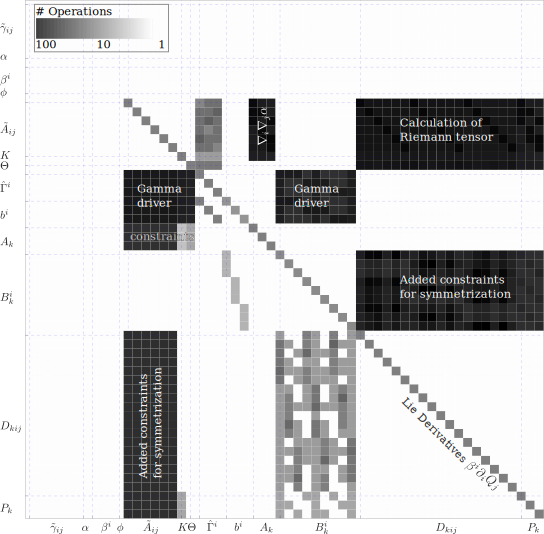
\includegraphics[width=\textwidth]{foccz4-cas/CCZ4-SystemMatrix-costs.pdf}
   	\caption[
     	FO-CCZ4 System matrix, evaluation costs (Mathematica sketch) \exclusive
   	]{
   		System matrix $\boldsymbol{A} \cdot \boldsymbol{n}$ with in
   		radial direction $\boldsymbol n = (1,1,1)$ as in
   		Figure~\protect\ref{fig:foccz4-sparsity}. Here, the color (shading) encodes the 
   		number
   		of basic operations
   		(additions and multiplications due to tensor contractions)
   		neccessary to compute the non-conservative product of that matrix element
   		on a logarithmic scale. The major blocks are labeled.
   		
   		The figure shows the two major cost drivers: The complex computation
   		of the Riemann (Ricci) tensor via the derivatives of the Christoffel
   		symbols via $D_{kij}$ (upper right) as well as the symmetrization
   		contributions which almost double the computational cost of the NCP.
   	}%
   	\label{fig:fo-ccz4-system-costs}
\end{figure}
%\todo[color=red]{Improve CCZ4 system cost image \ref{fig:fo-ccz4-system-costs}. It is really bad in the current shape.}

The \emph{costs} of a PDE system should measure its requirements in
runtime, memory and storage when being evaluated in a computer. Certainly,
in terms of memory requirements, due to the larger state vector, the costs
of the FO-CCZ4 system (59 unknowns) are certainly higher then of the SO-CCZ4
system (34 unknowns), which again is much more demanding then the original
ADM system (12 unknowns). When evaluated within the presented ADER-DG
scheme, the cost of the FO system will again be higher than the cost of
the SO system. This is due to the distinction between non-conservative product
(NCP) and source terms is made and the evaluation of the NCP takes place
several times within a timestep during the evaluation of the Riemann solver at
the cell boundaries. However, the FO system can also be evaluated with
traditional methods---Finite Differences and Runge Kutta (FDRK) where there
is only the right hand side differential operator.

The determination of
absolute costs is almost always inconclusive. For instance, the system
matrix, being a $\mathbb R^{n\times n}$ matrix, obviously grows with
$\mathcal O(n^2)$, where $n$ is the state vector size. A naive attemp is to
relate the cost ratio of FO/SO system to $58^2 / 34^2 \sim 2.9$. However,
this obviously does not even take the evaluation of tensors into account.
Figure~\ref{fig:foccz4-sparsity} already shows that the FO-CCZ4 system matrix
is sparse, and Figure~\ref{fig:fo-ccz4-system-costs} quantifies the differences
in terms of neccessary contractions to determine a certain element $A_{ij}$.
The amount of calculations varies over five orders of magnitude.
In other words, a few elements contribute to the overall number of
$\sim40,200$ elementary arithmetic operations (counting
special functions like $n^x$ and $x^n$ as one operation).
%\todo{FIGURE matrix \ref{fig:fo-ccz4-system-costs} needs adoption -- wie?}

\begin{margintable}[-6cm]
	\begin{tabular}{lcrr}
		\toprule
		Conf. & C & \#OP & $t$ [sec] \\
		\midrule
		\multirow{2}{*}{Dense}  & G & 8884 & 3.49 \\
		& I & 17761 & 8.92 \\
		\multirow{2}{*}{Sparse} & G & 5638 & 2.61  \\
		& I & 2757 & 6.14 \\
		\multirow{2}{*}{FullSimplify} & G & 4737 & 2.26  \\
		& I & 2730 & 4.42  \\
		\multirow{2}{*}{Optimized}  & G   & 5886 & 2.52  \\
		& I & 2821 & 5.77  \\
		\multirow{2}{*}{orderOpt} & G & 4141 & 2.76 \\
		& I & 1480 & 3.47 \\
		
		\bottomrule
	\end{tabular}
	\caption[
	Performance results of generating an optimized Z4 implementation
	]{
		\footnotesize % Fixme: "Table x.x" is in wrong fontsize
		Measuring the impact of differently ``optimized'' generated code
		to compute the NCP of the Z4 system. The first column describes
		the experiment, the second column shows which compiler was used
		to compile the Fortran code to assembler (G=GNU compiler,
		I=Intel compiler), \#OP indicates the number of assembler
		instructions which were generated while $t$ shows the serial
		runtime for $6\cdot10^6$ evaluations of the NCP with arbitrary
		but same state vectors (pseudo-randomly generated with the same seed).
		\\
		Experiments and interpretation are given in the main text.
	}\label{table:ccz4-implementation-optimization-minibenchmark}
\end{margintable}
%
A completely different measure is the number of assembler instructions
which have to be processed in order to compute a PDE function.
Table~\ref{table:ccz4-implementation-optimization-minibenchmark} provides
a small benchmark where different Fortran codes were generated by a CAS
(\code{Mathematica} and \code{Matlab} were used). In the first setup, all matrix elements
were specified, even the zero ones (\emph{Dense}), while in a second step,
the zero matrix elements were trivially removed (\emph{Sparse}). In a
subsequent step, a typical CAS ``simplification'' step (\emph{FullSimplify}) 
was performed, where algebraic expressions are brought in a form which requires
less evaluations (for instance by reducing polynomial expressions). The
\emph{Optimized} step further tried to store intermediate expressions to
variables, avoiding the need of computing certain expressions over and over
(trading memory for less arithmetic instructions). The \emph{orderedOpt} step
adopts a topological ordering of the required intermediate computations of the NCP
(adopting a task based paradigm), which should also reduce cache misses.

The results of this benchmarks are given as follows: While the number of
operations in principle can be decreased by one order of magnitude
(17kOP for the dense matrix vs. 1.4kOP for the topological ordered and
intermediate expressions computing version), the overall runtime stays in the
same regime and sophisticated algebraic transformations of the computation
order do not pay off.

The reasons for this are that optimizing for a small
number of assembler instructions is not the right measure at a CISC platform
\footnote{Complex instruction set computers (CISC) have machine instructions
  for various high level functions, which however can vary largely in execution
  time. In contrast, the presented measure is considerably more meaningful for
  reduced instruction set computers (RISC). In the current HPC landscape, CISC
  machines dominate, while there is however a trend for more RISC machines.},
while sophisticated vectorization units of the machine were
not used at all\footnote{
  The lack of vectorization in CAS-generated code stems from the fact that the tensorial algebra was not
  expound to the CAS in the chosen approach. While tensorial packages for CAS
  are in principle available (\cf Section~\vref{sec:symbolic-computing}),
  the freely available C/Fortran code generators from both Mathematica™ and
  Matlab™ do not generate optimized tensor contraction loops, such as discused in 
  Section~\ref{sec:implementing-ccz4-language}.
}. Therefore, a static analysis of code runtime is not meaningful.

%Furthermore, a benchmark run at a single core has little significance on
%a realistic multi core environment (\ie within an AMR code) where the full
%use of a compute node effects completely different memory and processor
%availability.


\subsection{Choosing the right language}\label{sec:implementing-ccz4-language}
There are several aspects that emerge when implementing large tensorial PDE systems.
First, as in physics, where the suitable choice of a coordinate system
can greatly reduce the complexity of a problem, or in mathematics, where
the transformation of a problem to another theory can provide new insights
and shortcuts, a suitable notation of the PDE system in a
computer-readable language/form reduces the abstraction neccessary from physics and
the equations as they are written on the paper.

The smallest common
demoninator in modern scientific programming languages is that of
\emph{linear algebra}, providing a compact language to manipulate
$n$-dimensional arrays in one expression (instead of looping over
vector or matrix axes). However, linear algebra misses a number of
features from differential geometry, for instance the distinction from
covariant and contravariant tensors. There is in fact the need for
a \emph{domain specific language} (DSL) which implements a minimum on
tensor algebra, \ie general style contractions (applying Einstein
sum convention).

As an example, an exemplaric contraction which shall compute $D^i$ is 
given,
\begin{equation}\label{eq:tensoralgebra-example}
D^i := A^{ik} B^{nm} C_{knm}
\end{equation}
with arbitary tensors $A,B,C$, where not even symmetries such as
$B^{nm} = B^{mn}$ shall be relevant at this point. While the mathematical
expression \eqref{eq:tensoralgebra-example} provides a clear instruction
how $D^i$ is defined by sums, thanks to associativity of addition and
multiplication, several evaluation strategies may lead to $D^i$. For
the FO-CCZ4 equations, using the \code{TensorTemplates} package
allows to write down this expression precisely as
\begin{equation}
\vec D = \TT{contract}{1,0}
 \left( A, \TT{trace}{0,2}\left(
   \TT{contract}{0,2}(B,C) \right) \right)
\end{equation}
This notation is declarative in a sense that it does not expose how
a contraction or trace is computed internally\footnote{
  The technical advantage (which comes on top of readability) of
  this abstraction is the fact that the implementation of the
  operation can be done efficiently by the compiler, for instance
  by exploting parallelization in terms of SIMD-vectorization.
} and it reveals the intermediate evaluation sequence as
\begin{equation}
A^{ik} B^{nm} C_{knm} \to A^{ik} E_{mkn} \to A^{ik} E_k \to D^i
\,.
\end{equation}
Providing efficient tensor algebra as a library is a whole branch of HPC
itself, and there is a plentitude of librarys available, however only a subset
of them deals with covariance\footnote{other covariance-aware tensor
libraries are for instance
the \code{Deal.II Library} \cite{Alzetta2018,Bangerth2007},
the \code{Tensor Contraction Engine} 
\cite{Baumgartner2005,Lam2011,Baumgartner2003},
\code{BARRACUDA} \cite{Nelson2015}, \code{InTensLi} \cite{Li2015}}.

\section{Benchmarks for solving FO-CCZ4 with ADER-DG}
%
\label{sec.tests}

In the following we present a battery of standard tests that explore the
ability of our formulation to carry out long-term stable evolutions of a
number of different spacetimes with increasing degree of curvature. If
not stated otherwise, in all of the tests we set initially $\Theta = 0$,
$\hat{\Gamma}^i = \tilde{\Gamma}^i$ and $b^i = 0$ and the HLLEM method is
used (Section~\ref{sec:holy-dg-scheme}).

In all tests the algebraic constraints on the
unit determinant of $\tilde{\gamma}_{ij}$, the zero trace of
$\tilde{A}_{ij}$ as well as the constraint $\tilde{\gamma}^{ij} D_{kij} =
0$ (which is a consequence of $|\tilde{\gamma}_{ij}|=1$) have all been
\textit{rigorously enforced} in the discrete solution
$\u_h(\boldsymbol{x},t^n)$ at the beginning of each timestep, but they
have \textit{not} been enforced during the computation of the spacetime
predictor $\q_h$. Note that the predictor $\q_h$ is only an auxiliary
quantity that is overwritten after each timestep and which has a role
similar to the evolution stage to the half timelevel in second-order 
MUSCL-Hancock type TVD finite-volume schemes.
%Note that in the very common case of a semidiscrete scheme evolved in
%time with a high-order Runge-Kutta (RK) time integrator, our choice
%corresponds to enforcing the constraints after a full timestep, but not
%in all the intermediate RK stages.
We therefore set $\tau \to \infty$ and thus neglect the corresponding
source terms. In tests involving black holes, the lower limit on the
lapse is set to be $\ln(\alpha) \geq -20$. We will use the notation $P_N$
to indicate an ADER-DG scheme using piecewise polynomials of degree $N$
to represent $\u_h$.

\subsection{Linearized gravitational-wave test}
%
\begin{marginfigure}
     \includegraphics[width=\textwidth]{foccz4-paper-official/LinearWave-P5-04-ADM.pdf}
        
     \includegraphics[width=\textwidth]{foccz4-paper-official/LinearWave-P5-04-waveform.pdf}
     \includegraphics[width=\textwidth]{foccz4-paper-official/LinearWave-P9-02-ADM.pdf}
     \includegraphics[width=\textwidth]{foccz4-paper-official/LinearWave-P9-02-waveform.pdf}
     \caption[
       Linearized GW test, 1D cuts and time series \ownPub{Dumbser2017}
     ]{Linearized gravitational-wave test using an ADER-DG $P_5$
      scheme with 4 elements (panels 1-2) and an ADER-DG $P_9$ scheme with
      only 2 elements (panels 3-4). The temporal evolution of the
      constraints (colour panels) is shown together with the waveform for
      the component $\tilde{A}_{22}$ of the traceless conformal extrinsic
      curvature after 1000 crossing times at time $t=1000$.}
    \label{fig.linearwave}
\end{marginfigure}
%
The first test problem is a simple one-dimensional wave-propagation test
problem in the linearized regime. The computational setup follows the one
suggested by in \cite{Alcubierre:2003pc}. The
computational domain is $\Omega = [-0.5,0.5]$ with periodic boundary
conditions in the $x$ direction and two simulations are run until a final
time of $t=1000$: \textit{(i)} a first one using 4 ADER-DG $P_5$ elements
(\ie a total number of 24 degrees of freedom) and \textit{(ii)} a second
one using only 2 ADER-DG $P_9$ elements (\ie only 20 degrees of
freedom). This test is run with the unlimited version of the ADER-DG
scheme. The exact solution of the metric of the problem is given by
%
\begin{align}
\label{eqn.lw.metric}
\d s^2 &= - \d t^2 + \d x^2 + (1+h) \d y^2 + (1-h) \d z^2\,, \\
\textnormal{with} \quad
h &:= \epsilon \sin \left( 2 \pi (x-t) \right)\,,
%
\end{align}
%
and the wave amplitude $\epsilon = 10^{-8}$ is chosen small enough in
order to stay in the linear regime, so that terms
$\mathcal{O}(\epsilon^2)$ can be neglected. Since the shift is zero in
the metric \eqref{eqn.lw.metric} ($\beta^i = 0$), we set $s=0$ in our
FO-CCZ4 system and furthermore harmonic slicing is used, \ie
$g(\alpha)=1$. We also set $K_0=0$, $c=0$, $e=2$ and use the 
\textit{undamped} version of the system, setting $\kappa_1 = \kappa_2 =
\kappa_3 = \eta = 0$. 
%We note that when setting $s=0$ and adopting a harmonic slicing it is
%necessary to choose $e > 1$ in order to get a strongly hyperbolic system,
%hence we use $e=2$. 
Using the metric \eqref{eqn.lw.metric}, the 
definition of the extrinsic curvature reduces to $K_{ij} = -
\tfrac{1}{2}\partial_t \gamma_{ij}/(\alpha)$, so that the various
components are given by $K_{xx} = K_{xy} = K_{xz} = K_{yz} = 0$, $K_{yy}
= -\halb \partial_t h$ and $K_{zz} = +\halb \partial_t h$. From this
information, the conformal factor $\phi$, the conformal spatial metric
$\tilde{\gamma}_{ij}$, the traceless conformal extrinsic curvature
$\tilde{A}_{ij}$ and all auxiliary variables can be computed by a direct
calculation according to their definitions.

In Fig. \ref{fig.linearwave} we report the temporal evolution of all ADM
constraints (Hamiltonian and momentum constraints) as well as the errors
of the algebraic constraints on the determinant of the conformal metric
and the error in the trace of $\tilde{A}_{ij}$ in both cases, \ie using
the ADER-DG $P_5$ and $P_9$ scheme. A comparison of the
extrinsic-curvature component $\tilde{A}_{22}$ with the exact solution is
also provided at the final time $t=1000$, showing overall an excellent
agreement between numerical and exact solution. The quality of the
results obtained with the ADER-DG schemes used in this paper, which are
uniformly high-order accurate in both space and time, is significantly
superior to the results shown in \cite{Alcubierre:2003pc} for the
same test problem using a finite difference scheme with much more grid
points (between 50 and 200) compared to the very coarse mesh containing
only 20 to 24 degrees of freedom used in our simulations. Note that a
fair comparison between high order finite-difference and DG schemes must
be made in terms of points per wavelength for finite-difference methods
and in degrees of freedom per wavelength for DG schemes.


\subsection{Gauge-wave test}
%
\begin{marginfigure}
	\includegraphics[width=\textwidth]{foccz4-paper-official/GaugeWaveA01-Waveform-phi.pdf}
	\includegraphics[width=\textwidth]{foccz4-paper-official/GaugeWaveA01-Waveform-K.pdf}

    \caption[
      Gauge-wave test, linear regime \ownPub{Dumbser2017}
    ]{Gauge-wave test case with amplitude $A=0.1$ using the
      undamped FO-CCZ4 system ($\kappa_1=\kappa_2=\kappa_3=0$) and
      improved cleaning speed $e=2$ with no damping $c=0$.
      Comparison with exact solution after $t=1000$.}
    \label{fig.gaugewave}
\end{marginfigure}
%
\begin{marginfigure}
    \includegraphics[width=\textwidth]{foccz4-paper-official/GaugeWaveA09-Waveform-phi.pdf}
    \includegraphics[width=\textwidth]{foccz4-paper-official/GaugeWaveA09-Waveform-K.pdf}
    \caption[
      Gauge-wave test, nonlinear regime \ownPub{Dumbser2017}
    ]{Highly nonlinear gauge-wave test case with very large
      amplitude $A=0.9$. Comparison of the wave form with the exact
      solution at time $t=10$ for an ADER-DG $P_5$ scheme and $100 \times
      10$ elements.}\label{fig.gauge.xxl}
\end{marginfigure}
%
Also this classical test problem has been taken from the collection of
standard tests of \cite{Alcubierre:2003pc}. The metric in this case
is given by
%
\begin{equation}
\begin{aligned}
\label{eqn.gw.metric}
\d s^2 &= - H(x,t) d t^2 + H(x,t) \d x^2 + \d y^2 + \d z^2\,, \\
\textnormal{with} \quad H(x,t) &:= 1-A\,\sin \left( 2\pi(x-t)
\right)\,.
\end{aligned}
\end{equation}
%
The metric \eqref{eqn.gw.metric} implies zero shift ($\beta^i = 0$),
hence we use once more $s=0$ together with harmonic slicing
$g(\alpha)=1$. Also for this test we employ the \textit{undamped} version
of the FO-CCZ4 system, setting $\kappa_1 = \kappa_2 = \kappa_3 = \eta =
0$. The computational domain in this case is two-dimensional, with $\Omega = [-0.5,0.5] \times
[-0.05, 0.05]$ with periodic boundary conditions in all directions. Since
$\beta^i = 0$, the extrinsic curvature is again given by $K_{ij} =
-\partial_t \gamma_{ij} / (2\alpha)$, \ie $K_{yy} = K_{zz} = K_{xy} =
K_{xz} = K_{yz} = 0$ and the remaining primary variables are
%
\begin{equation*}
\phi^2 = H^{-1/3}, \qquad  \alpha = \sqrt{H}, \qquad
K_{xx} = - \pi A\frac{\cos\left(2\pi(x-t)\right)}{\sqrt{1 - A\sin\left(2\pi(x-t)\right)}}.
\end{equation*}
We furthermore set $K_0=0$. The auxiliary variables can be
obtained from their definition via a straightforward calculation.

We first simulate this test problem with a perturbation amplitude of
$A=0.1$ until $t=1000$ with an unlimited ADER-DG $P_3$ scheme and using
$100 \times 10$ elements to cover the domain $\Omega$. We run this
physical setup twice, once with the default parameters $e=c=1$, according
to the original second order CCZ4 system \cite{Alic:2011a} and a
\textit{modified} setting with $e=2$ and $c=0$ to obtain an improved
cleaning of the Hamiltonian constraint. In both cases the system is
strongly hyperbolic.  The time evolution of the ADM constraints is
reported in Fig. \ref{fig.gaugewave}, showing only a very moderate growth
of the constraint $M_2$ that is sublinear in time and close to machine
precision. The other constraints $H$ and $M_1$ remain essentially
constant during the entire simulation.  We emphasize that we have used
the \textit{undamped} version of the FO-CCZ4 system, and nevertheless
obtain stable results, while the original second-order CCZ4 formulation
was reported to fail for this test problem in the undamped version, and
only the damped CCZ4 system was stable (see \cite{Alic:2011a} for
details). It is also worth recalling that both the first- and the
second-order formulation of the BSSNOK system fail for this test case
after a rather short time \cite{Alic:2011a, Brown2012}. In
Fig. \ref{fig.gaugewave} we also provide a direct comparison of the
solution after 1000 crossing times for the conformal factor $\phi$ as
well as for the trace of the extrinsic curvature $K$.
Note the overall 
very good agreement between the numerical solution and the exact
one. For the sake of clarity, in the plots of the waveforms we also
report the numerical error computed as the difference between the 
numerical solution and the exact solution at the final time $t=1000$. 
It can be clearly noticed from the computational results shown in Fig. 
\ref{fig.gaugewave} that the constraints and the phase errors in the 
waveforms are significantly smaller for the 
modified setting $e=2$, which may justify the use of a faster cleaning 
speed of the Hamiltonian constraint $e>1$ for \textit{purely numerical} 
purposes. In any case, our FO-CCZ4 system behaves well also with the 
default setting $e=c=1$, which is typically used in the standard 
second order CCZ4 system \cite{Alic:2011a}.

Since the gauge-wave test has a smooth nontrivial exact analytical
solution and is also valid in the nonlinear regime of the equations, we
can use it in order to perform a numerical convergence study. For this
purpose, we run the test again with different unlimited ADER-DG $P_N$
schemes on a sequence of successively refined meshes. To make the test
more difficult, we choose a very large perturbation amplitude of $A=0.9$,
which takes the system in the highly nonlinear regime, although in the
end the test consists only in a nonlinear re-parametrization of the flat
Minkowski spacetime. For thise case we use $c=0$ and $e=2$. We set the 
final simulation time to $t=10$ and continue using the \textit{undamped} 
version of the FO-CCZ4 system. 

\begin{table}[t]
	\caption[
	Gauge Wave convergence table \ownPub{Dumbser2017}
	]{Numerical convergence results for the large amplitude gauge wave
		test problem with $A=0.9$ at a final time of $t=10$.  The $L_2$
		errors and corresponding observed convergence order are reported for
		the variables $\phi$, $\alpha$ and $K$.
		Here, $\mathcal O({x})$ means the convergence order for $x$.
	}
	\centering\begin{adjustbox}{center,scale=0.9}
		%\renewcommand{\arraystretch}{1.0}
		\begin{tabular}{ccccccc}
			\hline
			$N_x \times N_y$ & ${L_2}$ error $\phi$ & $\mathcal{O}(\phi)$  & ${L_2}$ error $\alpha$ & $\mathcal{O}(\alpha)$  & ${L_2}$ error $K$ & $\mathcal{O}(K)$  \\
			\hline
			\multicolumn{7}{c}{$N=3$}   \\
			\hline
			$60 \times  6$  & 2.8663E-05 &     & 5.4876E-05 &      & 3.8469E-03 &      \\
			$80 \times  8$  & 1.0574E-05 & 3.5 & 2.2314E-05 & 3.1  & 7.0357E-04 & 5.9  \\
			$100\times 10$  & 3.8760E-06 & 4.5 & 8.0170E-06 & 4.6  & 2.3112E-04 & 5.0  \\
			$120\times 12$  & 1.6311E-06 & 4.7 & 3.2521E-06 & 4.9  & 9.7392E-05 & 4.7  \\
			\hline
			\multicolumn{7}{c}{$N=4$}   \\
			\hline
			$60 \times  6$  & 4.2966E-06 &     & 1.1408E-05 &      & 2.1910E-04 &      \\
			$80 \times  8$  & 8.9473E-07 & 5.5 & 2.3725E-06 & 5.5  & 5.0194E-05 & 5.1  \\
			$100\times 10$  & 2.5596E-07 & 5.6 & 6.8053E-07 & 5.6  & 1.5781E-05 & 5.2  \\
			$120\times 12$  & 9.0039E-08 & 5.7 & 2.4064E-07 & 5.7  & 6.1004E-06 & 5.2  \\
			\hline
			\multicolumn{7}{c}{$N=5$}   \\
			\hline
			$40 \times  4$  & 8.9305E-07 &     & 2.1971E-06 &      & 1.3614E-04 &      \\
			$60 \times  6$  & 5.2103E-08 & 7.0 & 1.2756E-07 & 7.0  & 5.9568E-06 & 7.7  \\
			$80 \times  8$  & 7.1947E-09 & 6.9 & 1.7348E-08 & 6.9  & 8.4259E-07 & 6.8  \\
			$100\times 10$  & 1.5357E-09 & 6.9 & 3.6421E-09 & 7.0  & 1.8093E-07 & 6.9  \\
			\hline
			\multicolumn{7}{c}{$N=7$}   \\
			\hline
			$30 \times 3$  & 1.7693E-08 &      & 3.9004E-08 &       & 6.3103E-06 &       \\
			$40 \times 4$  & 1.8387E-09 & 7.9  & 4.1751E-09 &  7.8  & 5.5791E-07 &  8.4  \\
			$60 \times 6$  & 6.2824E-11 & 8.3  & 1.4304E-10 &  8.3  & 2.1519E-08 &  8.0  \\
			$80 \times 8$  & 5.6521E-12 & 8.4  & 1.3455E-11 &  8.2  & 1.7085E-09 &  8.8  \\
			\hline
		\end{tabular}
	\end{adjustbox}
	\label{tab.conv1}
\end{table}

\begin{marginfigure}[-6cm]
	\includegraphics[width=\textwidth]{foccz4-paper-official/GaugeWaveE1-Constraints.pdf}
	\includegraphics[width=\textwidth]{foccz4-paper-official/GaugeWaveA01-Constraints.pdf}
	\caption[
	GaugeWave: Constraint evolution \ownPub{Dumbser2017}
	]{Growing of constraint violations during the Gauge Wave evolution.
		Note the logarithmic scale.}
	\label{fig.gaugewave2}
\end{marginfigure}

The $L_2$ error norms of the conformal factor $\phi$, the lapse $\alpha$ and
the trace of the extrinsic curvature $K$, together with the observed
order of accuracy of the different ADER-DG schemes are reported in Table
\ref{tab.conv1}. We observe essentially the expected order of accuracy of
the scheme for $N=3$ and $N=4$, while a superconvergence is observed for
$N=5$ and $N=7$. We think that this is due to the strong nonlinearities
of the PDE system appearing in the regime in which we run this test case
with $A=0.9$ and that some leading errors may be dominated by quadratic
terms in the metric and the conformal factor, which can lead to a faster
error decay than $N+1$ for \textit{coarse} meshes. However, we expect
that this superconvergence will disappear on sufficiently refined meshes;
but since the absolute errors are already getting close to machine
accuracy on the meshes used here, it is not possible to refine the mesh
much more with double-precision arithmetics, at least in the $N=7$ case.
For the ADER-DG $P_5$ scheme using $100 \times 10$ elements a comparison
between numerical and exact solution of the nonlinear waveforms for
$\phi$, $\alpha$, $K$ and $D_{xxx}$ is provided in Fig.
\ref{fig.gauge.xxl} at $t=10$, where we can note again an excellent
agreement between exact and numerical solution.

\subsection{Robust stability test}
%
\begin{marginfigure}
	\includegraphics[width=\textwidth]{foccz4-paper-official/RobustStabilityODE-10x10.pdf}
	\includegraphics[width=\textwidth]{foccz4-paper-official/RobustStabilityODE-80x80.pdf}
	\caption[
	Robust scability test \ownPub{Dumbser2017}
	]{Robust stability test case with Gamma-driver shift condition
		and $1+\log$ slicing with random initial perturbation of amplitude
		$10^{-7}/\rho^2$ in all quantities on a sequence of successively
		refined meshes on the unit square in 2D using an ADER-DG $P_3$
		scheme. Upper: $10\times10$ elements, corresponding to $40\times40$
		degrees of freedom ($\rho=1$). Lower: $80\times80$ elements, corresponding
		to $320\times320$ degrees of freedom ($\rho=8$). }
	\label{fig.robstab}
\end{marginfigure}
%
The  robust stability test is the last standard test problem
that we take from Ref. \cite{Alcubierre:2003pc}. While in the previous
test problems we have used a simple frozen shift condition $\partial_t
\beta^i = 0$ by setting $s=0$ in the FO-CCZ4 system, here we employ the
classical Gamma-driver shift condition. Furthermore, we employ the
$1+\log$ slicing condition, setting the slicing function to
$g(\alpha)=2/\alpha$ and the parameter $f$ of the Gamma driver to
$f=0.75$, which is also the typical value used for the BSSNOK system and
for the classical second-order CCZ4 system \cite{Alic:2011a}.
We further set $e=2$, $\kappa_1=\kappa_2=\kappa_3=0$, $K_0=0$,
$c=1$ and $\eta=0$.

As customary in this test, we start from the flat Minkowski metric.
We then add uniformly distributed \textit{random perturbations} to
\textit{all} quantities of the FO-CCZ4 system, \ie to all primary and
auxiliary variables and also to $\Theta$ and $\hat{\Gamma}^i$.  The
two-dimensional computational domain is $\Omega = [-0.5,0.5]^2$ and we
run different simulations with an unlimited ADER-DG $P_3$ scheme on four
successively refined meshes composed of $10 \rho \times 10 \rho$
elements, corresponding to $40 \rho \times 40 \rho$ degrees of freedom,
where $\rho \in \left\{ 1, 2, 4, 8 \right\}$ is the refinement factor.
The perturbation amplitude is $\epsilon = 10^{-7}/\rho^2$, which
corresponds to perturbation amplitudes that are three orders of magnitude
larger that those suggested in \cite{Alcubierre:2003pc}.

The time evolution of the ADM constraints is reported in Fig.
\ref{fig.robstab} for all four simulations. One can observe that after an
initial decay the constraints remain essentially constant in time for all
different grid resolutions, indicating that our FO-CCZ4 system indeed
passes the robust stability test with the standard Gamma driver and
$1+\log$ gauge conditions (see \cite{Cao:2012} for similar tests with the
Z4c system).



\subsection{Convergence tests on three-dimensional black-hole spacetimes}
\label{sec:convergence-bh3d}

In this test we consider the evolution of isolated Schwarzschild and Kerr
black holes in 3D Cartesian Kerr-Schild coordinates, with $M=1$ the mass
of the black hole and $a$ the dimensionless spin. The metric in these
coordinates is known analytically and thus the primary variables of our
evolution system are given by
%
\begin{equation}
  \alpha = S^{-\halb}\,, \qquad
	\beta^i = \frac{2 H}{S} l_i\,, \qquad
	\gamma_{ij} = \left( \begin{array}{ccc}
	 1 + 2 H l_x^2 & 2 H l_x l_y & 2 H l_x l_z \\
	 2 H l_x l_y & 1 + 2 H l_y^2  & 2 H l_y l_z \\
	 2 H l_x l_z & 2 H l_y l_z & 1 + 2 H l_z^2
	\end{array} \right)\,,
	\label{eqn.kerr.metric}
\end{equation}
%
with
%
\begin{equation*}
	 H := M \frac{r^3}{r^4 + a^2 z^2}\,, \qquad
	 S := 1 + 2 H\,, \qquad
	 l_x := \frac{r x + a y}{r^2 + a^2}\,, \qquad
	 l_y := \frac{r y - a x}{r^2 + a^2}\,, \qquad
	 l_z := \frac{z}{r}\,,
\end{equation*}
%
and
%
\begin{equation*}
r := \sqrt{ (x^2 + y^2 + z^2 - a^2)/2 + \sqrt{((x^2 + y^2 + z^2 -
    a^2)/2)^2 + z^2 a^2} }\,.
\end{equation*}
%
We furthermore use the fact that the solution is stationary, \ie
$\partial_t \gamma_{ij}=0$, hence the extrinsic curvature $K_{ij}$ is
computed as follows \cite{Rezzolla_book:2013}
%
\begin{equation}
K_{ij} = \frac{1}{2\alpha} \left( \nabla_i \beta_j + \nabla_j \beta_i
\right)\,.
\end{equation}
%

\begin{table*}[b]
	\caption[
	   Convergence results for different BH coordinates, 
	\ownPub{Dumbser2017}
	]{Numerical convergence results of FO-CCZ4 with simplified Gamma
		driver for the Schwarzschild black hole (left) and the Kerr black
		hole (right) in 3D Cartesian Kerr-Schild coordinates at a final time
		of $t=10$.  The $L_2$ errors and corresponding observed convergence
		order are reported for the variables $\phi$.}
	\label{tab.conv.bh}
	\vspace{.5cm}%
	\renewcommand{\arraystretch}{1.0}
	\begin{tabular}{cccccccccccc}
		\hline
		\multicolumn{6}{c}{\textbf{Schwarzschild black hole} ($a=0$)}   & \multicolumn{6}{c}{\textbf{Kerr black hole} ($a=0.9$)}   \\
		\hline
		$N_x$ & ${L_2}$ error $\phi$ & $\mathcal{O}(\phi)$  & $N_x$ & ${L_2}$ error $\phi$ & $\mathcal{O}(\phi)$  &
		$N_x$ & ${L_2}$ error $\phi$ & $\mathcal{O}(\phi)$  & $N_x$ & ${L_2}$ error $\phi$ & $\mathcal{O}(\phi)$  \\
		\hline
		\multicolumn{3}{c}{$N=3$}  &  \multicolumn{3}{c}{$N=5$}    &
		\multicolumn{3}{c}{$N=3$}  &  \multicolumn{3}{c}{$N=5$}    \\
		\hline
		10	& 9.9982E-06	&     &   5 & 2.1837E-06 &     & 10	& 1.4270E-05	&     &   5 & 2.6679E-06 &     \\
		15	& 1.8439E-06	& 4.2	&  10 & 2.8327E-08 & 6.3 & 15	& 2.8279E-06	& 4.0 &  10 & 6.5136E-08 & 5.4    \\
		20	& 5.8521E-07	& 4.0	&  15 & 2.3649E-09 & 6.1 & 20	& 8.9487E-07	& 4.0 &  15 & 6.0944E-09 & 5.8    \\
		25	& 2.4322E-07	& 3.9	&  20 & 4.1176E-10 & 6.1 & 25	& 3.6468E-07	& 4.0 &  20 & 1.1087E-09 & 5.9    \\
		\hline
	\end{tabular}
\end{table*}
%
The function $K_0$ is chosen as $K_0 = \left( K - \beta^k \partial_k
\alpha \right)/{\left(\alpha^2 g(\alpha)\right)}$, so that $ \partial_t
\alpha = 0$ and in this test the Gamma-driver shift condition is
simplified to $\partial_t \beta^i = f b^i$, $\partial_t B_k^i = f
\partial_k b^i$ and $\partial_t b^i = \partial_t \hat{\Gamma}^i$, with
the consequence that the above exact solution corresponds to a stationary
solution of the FO-CCZ4 system. In other words, we remove the advection
terms from the evolution equations of the shift $\beta^i$ and the
variable $b^i$ (see also \cite{Alcubierre:2008}). The conformal factor
$\phi$ and the auxiliary variables can be computed according to their
definition. The computational domain is chosen as $\Omega = [1,5]^3 \,
M^3$, and the exact solution given by the initial condition is imposed on
all boundaries in all variables at all times. Note that this choice of
boundary conditions is appropriate to study convergence since the exact
solution is also a stationary solution of our PDE system. Note also that
the black hole is centered at $x=y=z=0$, so that we evolve only a section
of the domain offset from the singularity, but encompassing regions both
inside and outside of the event horizon; this effectively amounts to
employing an excision of the black-hole interior.  We furthermore set
$e=2$, $c=1$, $\eta=0$, and consider the undamped CCZ4 system with the
$1+\log$ slicing, \ie we set $\kappa_1 = \kappa_2 = \kappa_3 = 0$,
$f=0.75$ and $g(\alpha)=2 / \alpha$.

The simulations were performed with different ADER-DG schemes on a
sequence of successively refined meshes until a final time of
$t=10\,M$. The Rusanov method is used as approximate Riemann solver at
the element interfaces. In the case of the Schwarzschild black hole we
use $a=0$, while for the Kerr black hole we set $a=0.9$. The
corresponding numerical convergence rates are reported for both cases in
Table \ref{tab.conv.bh}, where we observe that the designed order of
accuracy $N+1$ of our high-order fully-discrete one-step ADER-DG schemes
has been properly reached.


\subsection{Evolution of a single puncture black hole}
\label{sec.single.punctures}

We next have applied the FO-CCZ4 formulation to a single puncture black
hole \cite{Brandt97b} with mass $M=1$ and dimensionless spin $a=0$
located at the origin of a three-dimensional computational domain $\Omega
= [-150,150]^3 \, M^3$ with periodic boundary conditions on all
boundaries. The
domain is discretized with an AMR mesh with grid spacing $\Delta x =
\Delta y = \Delta z = 2.5\,M$ within the inner box $\Omega_b = [-15,15]^3
\, M^3$, while $\Delta x = \Delta y = \Delta z = 7.5\,M$ is used in the
outer part of the domain. In the innermost zone $\Omega_l = [-3,3]^3 \,
M^3$ the third-order subcell ADER-WENO finite-volume limiter is activated
throughout the entire simulation. For details on the AMR framework and
the subcell finite-volume limiter we refer the interested reader again to
\cite{Dumbser2014,Zanotti2015c,Zanotti2015b}. We also stress that this
simulation can be run only after activating the finite-volume subcell
limiter, since a robust scheme is needed in order to deal with the
puncture singularity. Without such a limiter, \ie with a pure DG scheme,
the code crashes after a few timesteps since the high-order unlimited DG
scheme is \textit{not} robust enough to deal with the puncture metric. In
our simulation we use an ADER-DG $P_3$ scheme ($N=3$), which leads to
$2N+1 = 7$ finite-volume subcells per DG element, \ie the effective mesh
spacing in terms of points (cell averages) inside the domain $\Omega_l$
is $\Delta x = \Delta y = \Delta z = 0.357\,M$.  Note that we set up the
mesh so that the puncture is located at the boundary of the DG elements;
given the location of the degrees of freedom in the subcell grid, no grid 
point coincides with the puncture.
We set the CCZ4 parameters to $\kappa_1 = 0.1$, $\kappa_2=0$, $\kappa_3 =
0.5$ and $\eta=0$. The constant $\mu$ accounting for the second-order
ordering constraints in the evolution of $B^i_k$ is set to $\mu=1/5$,
while for this test we use $c=1$, $f=0.75$ and $e=1$ to be as close as 
possible to a standard second-order CCZ4 formulation, where the cleaning 
of the Hamiltonian constraint is done at the speed of light.

\begin{marginfigure}
	\includegraphics[width=\textwidth]{foccz4-paper-official/SinglePunctureBH-ODE-eta0.pdf}
	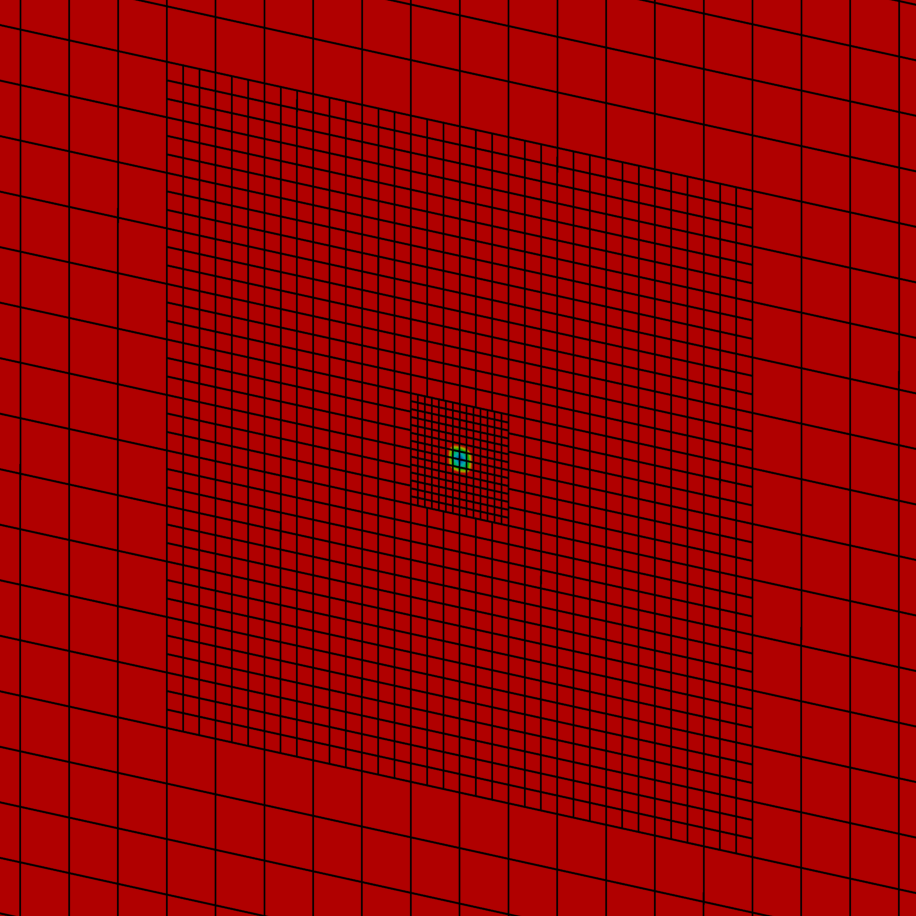
\includegraphics[width=\textwidth]{foccz4-paper-amended/OnePunctureODE-zoom.png}
	\caption[
	Single puncture black hole, constraint evolution \ownPub{Dumbser2017}
	]{Time evolution of the ADM constraints for the single
		puncture black hole using an ADER-DG $P_3$ scheme with AMR and
		ADER-WENO subcell finite-volume limiter until $t=1000$ (left). Color
		contours for the lapse at $t=200$ and grid setup showing the domain
		$\Omega$, the refined box $\Omega_b$ and the zone with active subcell
		finite-volume limiter $\Omega_l$ (center). Zoom into the center
		region at $t=200$ with color contours for $\alpha$ (right).}
	\label{fig.puncture}
\end{marginfigure}

% 
The initial metric and lapse are provided by the \texttt{TwoPunctures}
initial data code \cite{Ansorg:2004ds} (part of the \code{Einstein Toolkit}
 \cite{loeffler_2011_et}). Explicitly, the lapse is set initially
to
\begin{equation}
    \alpha = \halb \left(\frac{1-\halb \left({M}/{r^*}\right)}{1+\halb
        \left({M}/{r^*}\right)}+1\right)\,,
\end{equation}
%
where $r^*:=(r^4+10^{-24})^{\frac{1}{4}}$ and $r$ is the coordinate
distance of a grid point from the puncture. The auxiliary quantities
(which are spatial derivatives of the primary quantities) are obtained
via a simple fourth order central finite difference applied to the
primary variables $\alpha$ and $\gamma_{ij}$. Initially the shift and the
extrinsic curvature are set to zero, \ie $\beta^i = 0$ and $K_{ij}=0$.

The evolution was carried out until a final time of $t=1000\,M$ and
Fig. \ref{fig.puncture} reports the evolution of the average $L_2$ error
of the ADM constraints, which we define as
%
\begin{equation*}
\overline{L}_2 = \sqrt{ \frac{\int_\Omega \epsilon^2
    \d\boldsymbol{x}}{\int_\Omega d\boldsymbol{x} } }\,,
\end{equation*}
%
where $\epsilon$ denotes the local error of each of the ADM quantities,
\ie Hamiltonian $H$ and momentum constraints $M_i$. In Fig. \ref{fig.puncture}
also a view of the 3D grid setup is shown together with a zoom into the center 
region with the contour colors of the lapse function at a time of $t=200\,M$.  
%
It is probably worth recalling that, to the best of our knowledge, these
are the first results obtained for a puncture black-hole spacetime using
a fully three-dimensional DG finite-element method with AMR and LTS.
Previous results obtained with high-order DG schemes for black-hole
spacetimes were essentially limited to the one-dimensional case 
\cite{field10, Brown2012, Miller2016}.

\newpage
\subsection{Preliminary results for moving punctures}\label{sec.movpunct}
\begin{marginfigure}
	\includegraphics[width=\textwidth]{foccz4-paper-official/TPRusanov-t00.pdf} 
	\\[.3em]
	\includegraphics[width=\textwidth]{foccz4-paper-official/TPRusanov-t07.pdf}
	\\[.3em]
	\includegraphics[width=\textwidth]{foccz4-paper-official/TPRusanov-t10.pdf}
	\\[.3em]
	\includegraphics[width=\textwidth]{foccz4-paper-official/TPRusanov-t15.pdf}
	\caption[
	  BH-BH head-on collision, time evolution snapshots, \ownPub{Dumbser2017}
	]{Time evolution of the contour surfaces of the lapse $\alpha$
		and the shift vector $\beta^i$ for the head-on collision of two
		puncture black holes of equal mass $M=1$ at times
		$t=0,\,5,\,7,\,8,\,10\,M$ and $t=15\,M$, from top left to bottom
		right.}
	\label{fig.twopunctures}
\end{marginfigure}

The last test considered is a preliminary application of the FO-CCZ4
system to a binary system of two moving punctures. In particular, we
consider a head-on collision of two nonrotating black holes of equal mass
$M=1$ with zero linear momentum initially located at $\boldsymbol{x}^- =
(-1,0,0)$ and $\boldsymbol{x}^+ = (+1,0,0)$. The three-dimensional
computational domain is given by $\Omega = [-25,25]^3 \, M^3$ and flat
Minkowski spacetime is imposed as boundary condition everywhere.  The
CCZ4 parameters are set to $\kappa_1 = 0.1$, $\kappa_2=0$, $\kappa_3 =
0.5$, $\eta=0$ and furthermore we choose $c=1$, $e=1$, $f=1$ and $\mu=1/5$.
Again, the initial metric and the lapse are provided by the
\texttt{TwoPunctures} initial data code \cite{Ansorg:2004ds}, with the lapse
set initially to
\begin{equation}
    \alpha =
    \halb\left(
    \frac{1-\halb\left({m_-}/{r_-^*}\right)-\halb\left({m_+}/{r_+^*}\right)}
    {1+\halb\left({m_-}/{r_-^*}\right)+\halb\left({m_+}/{r_+^*}\right)}
    +1  \right)\,,
\end{equation}
where $r^*_-$ and $r^*_+$ are the coordinate distances of a grid point
from either puncture (defined analogously to the previous section) and
$m_-$ and $m_+$ are the  bare masses of the two black holes (see
\cite{Ansorg:2004ds}) and in this case they are equal. The auxiliary
quantities are computed from the primary variables via a fourth-order
central finite-difference method. We use the simple and robust Rusanov
method as approximate Riemann solver on the element boundaries.  The
shift and extrinsic curvature are initially set to $\beta^i = 0$ and
$K_{ij}=0$.

The domain is discretized with an AMR mesh of mesh spacing $\Delta x =
\Delta y = \Delta z = 5/12\,M$ within the inner box $\Omega_b =
       [-2.5,2.5]^3 \, M^3$, while $\Delta x = \Delta y = \Delta z =
       1.25\,M$ is used in the outer part of the domain. In the innermost
       zone $\Omega_l = [-5/3,5/3]^3 \, M^3$ the third-order subcell
       ADER-WENO finite-volume limiter is activated throughout the entire
       simulation. As for a single puncture, we use an ADER-DG $P_3$
       scheme ($N=3$), whose $2N+1 = 7$ finite-volume subcells lead to an
       effective mesh spacing inside the domain $\Omega_l$ of $\Delta x =
       \Delta y = \Delta z = 0.0595$. Once again we remark that the use
       of the finite-volume subcell limiter is essential in order to
       obtain a stable evolution.

The simulation is run until a final time of $t=60\,M$ and the evolution
of the contour surfaces of the lapse and the shift vector are reported in
Fig. \ref{fig.twopunctures}. The contour surfaces of the conformal factor
at the final time as well as the evolution of the ADM constraints are
depicted in Fig. \ref{fig.twopunctures.adm}. Clearly, no sign of growth
in the violation of the constraints appears after the two punctures have
merged at $t\simeq 10\,M$.

Although these results are meant mostly as a proof-of-concept rather than
as a realistic modelling of the inspiral and merger on binary black-hole
systems, they provide convincing evidence that binary systems of puncture
black holes can be evolved stably with our path-conservative ADER-DG
scheme with ADER-WENO subcell finite-volume limiter on AMR grids based on
the FO-CCZ4 formulation proposed here. A more detailed and systematic
investigation, which includes the emission of gravitational waves from
binary systems of rotating black holes in quasi-circular orbits 
\cite{Alic:2011a}, will be the subject of future work.

\section{Summary}
\begin{marginfigure}
	\includegraphics[width=\textwidth]{foccz4-paper-official/TPRusanov-phi-t34.pdf}
	\includegraphics[width=\textwidth]{foccz4-paper-official/TPCollisionADM.pdf}
	\caption[
	BH Head-on collision, final snapshot and error time evolution, 
	\ownPub{Dumbser2017}
	]{Head-on collision of two puncture black holes: contour
		surfaces of the conformal factor $\phi$ at time $t=34\,M$ after the
		merger (left) and time evolution of the ADM constraints (right).
		The curves for the second and third momentum constraint almost
		coincide. }
	\label{fig.twopunctures.adm}
\end{marginfigure}

In Chapter~\ref{chapter:gr}, the evolution from classical 3+1 formulation of
Einsteins field equations over BSSNOK and the Z4 family to CCZ4 was passed. The
rewriting of CCZ4 to a first order formulation was discussed in detail and
remarks on mathematical and computer-science (implementation) related points
were made. Afterwards, the ADER-DG scheme from Section~\ref{sec:dg} was applied
in order to demonstrate the correctness of the PDE and applicability of the
scheme in a couple of standard numerical relativity testbeds. Some of these
tests are especially remarkable, since these are the first simulations of 
black-hole spacetimes ever performed in three spatial dimensions with high-order
discontinous galerkin methods. However, all examples shown in this sections
were restricted to ``vacuum solutions'' of Einsteins equations, where the
matter contribution $T_{\mu\nu}$ is exactly zero. Chapter~\vref{chapter:hydro}
is dedicated to discuss the powerful and widespread theory of hydrodynamics 
for a non-zero assignment of $T_{\mu\nu}$ in the given equations, while 
providing its standalone evolution equations for individual quantities
resembling the energy momentum tensor.

